\documentclass[onecolumn]{article}

%% ====================================================================
%% Packages (identical to methodology.tex)
%% ====================================================================
\usepackage[T1]{fontenc}
\usepackage[utf8]{inputenc}
\usepackage{textcomp}
\usepackage{graphicx}
\usepackage{url}
\usepackage{amsmath}
\usepackage{amssymb}
\usepackage{amsfonts}
\usepackage{xcolor}
\usepackage{array}
\usepackage{float}
\usepackage{subcaption}
\usepackage{caption}
\usepackage{booktabs}
\usepackage{geometry}
\usepackage{multirow}
\usepackage{placeins}
\usepackage{hyperref}
\geometry{margin=2.5cm}
\usepackage{authblk}
\usepackage{enumitem}
\usepackage{algorithm}
\usepackage{algpseudocode}
\usepackage{CJK}
\usepackage{xr-hyper}
\externaldocument{methodology}   %% cross-ref labels from main body

\title{Supplementary 1: Denoised Pairdata and LoRA Finetuning (v0.7.5, pairdata v2)}
\author[1]{Takato Yasuno}
\date{}

\begin{document}
\renewcommand{\figurename}{Figure}
\renewcommand{\tablename}{Table}
\maketitle

\section*{Supplementary 1: Denoised Pairdata and LoRA Finetuning (v0.7.5, pairdata v2)}
\label{sec:supplementary1}

%%--------------------------------------------------------------------
\subsection*{S.1 Motivation}
%%--------------------------------------------------------------------

Several failure modes identified in the main study (Section~\ref{sec:discussion})
can be attributed to out-of-scope content in the pairdata\_v1 ground truth texts.
Specifically: (i)~mode collapse toward dominant components
(Main Girder 100\,\%, Rebar Exposure 99.6\,\%, Spalling 98.6\,\% of all predictions;
see Section~\ref{sec:disc_mode_collapse}),
(ii)~degradation of cosine similarity at the 4\,k scale
(3\,k: $\rho=0.6909$ vs.\ 4\,k: $\rho=0.6739$), and
(iii)~score saturation (all 727 PASS samples converging to Level~3, score~$=0.54$).

The single-image VLM aspect of the pipeline (Aspect~1, Section~\ref{sec:scope})
is limited to what is visible at one point in time.
However, pairdata\_v1 inspection texts routinely contain two categories of
out-of-scope clauses:
\begin{itemize}
  \item \textbf{Category~A ---  Temporal comparison:}
        Clauses referring to changes since a previous inspection
        (\textit{e.g.}, \begin{CJK}{UTF8}{ipxm}前回より進行\end{CJK}: ``progressed since last inspection'').
        These require at least two images separated in time and are unlearnable
        from a single frame.
  \item \textbf{Category~B --- Maintenance recommendations:}
        Prescriptive clauses specifying repair methods or urgency
        (\textit{e.g.}, \begin{CJK}{UTF8}{ipxm}早期に補修が必要\end{CJK}: ``early repair required'').
        These depend on bridge-level management metadata unavailable to the VLM.
\end{itemize}

\noindent
Removing these clauses at the sentence level---while leaving the structural
damage descriptions intact---yields \textbf{pairdata\_v2}.
The same denoising is applied to both the training pool and the test-set
ground truth, so that training signals and evaluation targets are aligned.
Direct numerical comparison with v0.3/v0.6.3 results (pairdata\_v1 GT) is
not applicable by design.

%%--------------------------------------------------------------------
\subsection*{S.2 Noise Pattern Definition}
%%--------------------------------------------------------------------

Denoising is implemented as a sentence-level filter:
each inspection text is split on the Japanese full stop (\begin{CJK}{UTF8}{ipxm}。\end{CJK}) and each
resulting clause is tested against two regular-expression sets.
Matching clauses are discarded; the remainder is re-joined.

\begin{table}[h]
\centering
\caption{Out-of-scope sentence patterns removed in pairdata\_v2.}
\label{tab:noise_patterns}
\small
\begin{tabular}{ll p{5.5cm} p{5cm}}
\toprule
\textbf{Cat.} & \textbf{Label} & \textbf{Regex pattern (Japanese)} & \textbf{Meaning (English)} \\
\midrule
A & Temporal & \begin{CJK}{UTF8}{ipxm}\texttt{前回(より|から|の|点検|調査)}\end{CJK} & previous inspection/survey \\
A & Temporal & \begin{CJK}{UTF8}{ipxm}\texttt{前年(より|から|の)}\end{CJK} & previous year (from/than/of) \\
A & Temporal & \begin{CJK}{UTF8}{ipxm}\texttt{経時(的|変化)}\end{CJK} & time-dependent change \\
A & Temporal & \begin{CJK}{UTF8}{ipxm}\texttt{新たに.{0,15}(発生|出現)}\end{CJK} & newly occurred/appeared \\
\midrule
B & Maintenance & \begin{CJK}{UTF8}{ipxm}\texttt{補修(が|を|は)?(必要|要する|望ましい|検討)}\end{CJK} & repair required/recommended \\
B & Maintenance & \begin{CJK}{UTF8}{ipxm}\texttt{予防保全}\end{CJK} & preventive maintenance \\
B & Maintenance & \begin{CJK}{UTF8}{ipxm}\texttt{対策(が|を)?(必要|要する|講じ)}\end{CJK} & countermeasure required/taken \\
B & Maintenance & \begin{CJK}{UTF8}{ipxm}\texttt{措置(が|を)?(必要|要する)}\end{CJK} & measures required \\
B & Maintenance & \begin{CJK}{UTF8}{ipxm}\texttt{経過観察(が|を)?(必要|要する)}\end{CJK} & follow-up monitoring required \\
B & Maintenance & \begin{CJK}{UTF8}{ipxm}\texttt{早(期|急)に.{0,15}(補修|対策|措置|点検|確認)}\end{CJK} & urgent repair/action required \\
B & Maintenance & \begin{CJK}{UTF8}{ipxm}\texttt{維持管理計画}\end{CJK} & maintenance management plan \\
B & Maintenance & \begin{CJK}{UTF8}{ipxm}\texttt{補修工法|補修方法}\end{CJK} & repair method/technique \\
\bottomrule
\end{tabular}
\end{table}

%%--------------------------------------------------------------------
\subsection*{S.3 Pairdata Statistics Comparison}
\label{sec:pairdata_comparison}
%%--------------------------------------------------------------------

Table~\ref{tab:pairdata_stats} compares the two ground-truth corpora.
Denoising reduced total pool size by $\approx$1\% (9,880 $\to$ 9,785 rows)
while shortening mean text length by 16\% (93.7 $\to$ 78.5 chars),
confirming that out-of-scope clauses were disproportionately verbose.
Rows fully emptied after denoising (31 of 4,378 affected, 0.7\%) were
excluded from both training and evaluation.

\begin{table}[h]
\centering
\caption{pairdata\_v1 vs.\ pairdata\_v2: dataset statistics.}
\label{tab:pairdata_stats}
\small
\begin{tabular}{l r r}
\toprule
\textbf{Metric} & \textbf{pairdata\_v1} & \textbf{pairdata\_v2} \\
\midrule
\multicolumn{3}{l}{\textit{Pool size}} \\
\quad Total rows (after filtering) & 9,880 & 9,785 \\
\quad Retention rate (\%) & 90.6 & 89.7 \\
\midrule
\multicolumn{3}{l}{\textit{Denoising (pairdata\_v1 $\to$ v2)}} \\
\quad Cat.\ A sentences removed & --- & 2,124 \\
\quad Cat.\ B sentences removed & --- & 3,022 \\
\quad Total sentences removed & --- & 5,146 \\
\quad Rows with $\geq$1 sentence removed & --- & 4,378 \\
\quad Rows fully emptied & --- & 31 \\
\midrule
\multicolumn{3}{l}{\textit{Test-set text length (chars, $n=800$)}} \\
\quad Mean & 93.7 & 78.5 \\
\quad Median & 86.0 & 71.0 \\
\quad Std dev & 47.9 & 42.7 \\
\quad Min / Max & 15 / 291 & 15 / 241 \\
\bottomrule
\end{tabular}
\end{table}

%%--------------------------------------------------------------------
\subsection*{S.4 Input Image Resolution Study (v0.7.1)}
\label{sec:s4_image_size}
%%--------------------------------------------------------------------

\subsubsection*{Motivation}

LLaVA-1.5-7B employs a CLIP ViT-L/14-336 vision encoder pretrained at
$336\times336$ pixels~\cite{liu2024llava}.
When training images are supplied at arbitrary resolutions, the model's
internal processor forcibly rescales them to this native size, introducing
resampling artefacts into the patch embeddings.
We hypothesise that pre-standardising training images to the encoder's
native resolution ($336\times336$) reduces artefact noise and yields
higher fine-tuning accuracy.

\subsubsection*{Preprocessing Pipeline}

Starting from 10{,}789 raw bridge inspection photographs
(width: $\mu=1394$, range $867$--$5013$\,px;
height: $\mu=1042$, range $651$--$2501$\,px),
we applied the following three-stage pipeline:

\begin{enumerate}
  \item \textbf{Long-side resize.}
        Each image is resized so that $\max(W,H)=1024$\,px with
        aspect ratio preserved (\texttt{Lanczos}, JPEG quality~92).
        Output: \texttt{data/inspect\_images\_v2/} (10{,}789 images).

  \item \textbf{Manual noise removal.}
        A human reviewer inspected \texttt{inspect\_images\_v2/} and
        removed 121~images classified as blueprints, blank sheets, or
        severely corrupted photographs.
        Remaining: \textbf{10{,}668 images}.

  \item \textbf{Center-crop and resize.}
        Each image is cropped to a $\min(W,H)\times\min(W,H)$ square
        anchored at the image centre, then resized to two target
        resolutions using \texttt{PIL.Image.LANCZOS}:
        \begin{itemize}
          \item $336\times336$\,px $\rightarrow$
                \texttt{data/inspect\_images\_336/}
                (avg.\ $0.034$\,MB, JPEG quality~92)
          \item $448\times448$\,px $\rightarrow$
                \texttt{data/inspect\_images\_448/}
                (avg.\ $0.060$\,MB, JPEG quality~92)
        \end{itemize}
\end{enumerate}

Center-cropping (rather than pad-and-resize) was chosen because
bridge damage sites are typically centred in the field of view;
padding would introduce uniform black borders that divert the
vision encoder's attention from damage regions.

\subsubsection*{Experimental Design}

Three input datasets were constructed from the same 1{,}000-sample
training split (\texttt{train\_1k.csv}), differing only in the image source:

\begin{table}[h]
\centering
\caption{Input datasets compared in the S.4 image resolution study.}
\label{tab:s4_datasets}
\small
\begin{tabular}{llll}
\toprule
\textbf{Dataset} & \textbf{Image source} & \textbf{Resolution} & \textbf{Note} \\
\midrule
pairdata\_v2-1 & \texttt{rank\_c\_images\_n10789} & Variable (original) & Baseline \\
pairdata\_v2-2 & \texttt{inspect\_images\_336}   & $336\times336$\,px  & Native CLIP size \\
pairdata\_v2-3 & \texttt{inspect\_images\_448}   & $448\times448$\,px  & High-resolution option \\
\bottomrule
\end{tabular}
\end{table}

\noindent
All other hyperparameters were held constant:
LoRA $r{=}32$, $\alpha{=}64$, dropout $0.05$;
3~epochs; LR $2\times10^{-4}$ (cosine schedule);
batch size~4, gradient accumulation~4 (effective batch~16);
BF16 mixed precision; RTX~4060~Ti 16\,GB.
Ten training samples were skipped for pairdata\_v2-2 and pairdata\_v2-3
because the corresponding images were among the 121 manually removed in
Step~2 above (990 valid samples).

\subsubsection*{Results}

\begin{table}[h]
\centering
\caption{QLoRA 1k-scale training results by input image resolution.}
\label{tab:s4_results}
\small
\begin{tabular}{lllll}
\toprule
\textbf{Dataset} & \textbf{Training Time} & \textbf{eval\_loss} &
\textbf{eval Token Acc.} & \textbf{$\Delta$ Acc.\ vs.\ v2-1} \\
\midrule
pairdata\_v2-1 (variable) & 1\,h\,34\,m\,53\,s & 3.189 & 89.5\,\% & --- \\
\textbf{pairdata\_v2-2 ($336$\,px)} & \textbf{1\,h\,21\,m\,46\,s} & 3.194 & \textbf{90.1\,\%} & $+0.6$\,pt \\
pairdata\_v2-3 ($448$\,px) & 1\,h\,21\,m\,57\,s & 3.202 & 89.9\,\% & $+0.4$\,pt \\
\bottomrule
\end{tabular}
\end{table}

\subsubsection*{Discussion}

The $336\times336$ dataset (pairdata\_v2-2) achieves the highest
token accuracy ($90.1$\,\%) with the shortest training time
($1$\,h\,$21$\,m\,$46$\,s, a $13.9$\,\% reduction relative to the
variable-resolution baseline).
The training time reduction is attributable to uniform tensor shapes
enabling more efficient GPU memory coalescing.

The $448\times448$ dataset shows no accuracy advantage over $336\times336$
despite a $76$\,\% larger mean file size.
This result is consistent with the hypothesis that the CLIP
ViT-L/14-336 encoder constitutes the binding resolution constraint:
supplying images at $448$\,px does not provide additional information
to the frozen vision encoder because it immediately rescales them
to its $336$\,px patch grid.

The slightly higher \texttt{eval\_loss} for pairdata\_v2-2 ($3.194$)
versus pairdata\_v2-1 ($3.189$) is not contradicted by the accuracy
result; token accuracy is the more informative metric because it
directly measures next-token prediction success rather than the
log-probability of the exact reference tokens.

\subsubsection*{Recommendation}

Based on these results, \textbf{$336\times336$ center-cropped images
are adopted as the default for all subsequent v0.7 training runs}
(2k, 3k, 4k scales).
The configuration files \texttt{config.yaml} and
\texttt{train\_v07\_qlora.py} have been updated accordingly.

%%--------------------------------------------------------------------
\subsection*{S.5 Progressive Retraining Results (pairdata\_v2)}
%%--------------------------------------------------------------------

\subsubsection*{Setup}

Following the same progressive schedule used in the main study
(Section~\ref{sec:progressive}), four model variants were trained
on increasing subsets of the denoised pairdata\_v2 corpus:
1\,k, 2\,k, 3\,k, and 4\,k paired samples.
All runs shared the same hyperparameters (LoRA $r{=}32$, $\alpha{=}64$,
dropout $0.05$; 3~epochs; LR $2\times10^{-4}$ cosine schedule; batch
size~4, gradient accumulation~4; BF16; RTX~4060~Ti 16\,GB) and the same
image source (\texttt{data/inspect\_images\_336/}, $336\times336$\,px
center-crop; see S.4).
Each scale was split 80\,/\,20 into training and validation sets;
evaluation was performed every 100~gradient-update steps using
teacher-forcing token accuracy and cross-entropy loss.

Note: these results are \emph{not} directly comparable to
Table~\ref{tab:training_results} because both training texts and
evaluation references now use the denoised pairdata\_v2 ground truth.

\subsubsection*{Results}

\begin{table}[h]
\centering
\caption{%
  Progressive QLoRA training on pairdata\_v2 (denoised, inspect\_images\_336).
  Token accuracy and eval loss are reported at the final epoch (epoch~3).
  Values in parentheses show the result at epoch~1 where available.}
\label{tab:s4_progressive}
\small
\begin{tabular}{lrrrllc}
\toprule
\textbf{Scale} &
\textbf{Train} &
\textbf{Val} &
\textbf{Skip} &
\textbf{Duration} &
\textbf{eval loss} &
\textbf{Token acc.\ (eval)} \\
\midrule
1\,k & 792  & 198 & 10  & 1\,h\,21\,m & 3.194 & 90.1\,\% \\
2\,k & 1579 & 395 & 26  & 2\,h\,56\,m & 3.151 & 98.7\,\% \\
3\,k & 2374 & 594 & 32  & 4\,h\,24\,m & 3.135 & 99.0\,\% \\
4\,k & 3168 & 792 & 40  & 5\,h\,55\,m & 3.125 & 99.2\,\% \\
\bottomrule
\end{tabular}
\end{table}

\noindent
\textit{Skip} denotes training samples skipped because the corresponding
image was removed during manual noise filtering (S.2).

\subsubsection*{Per-Epoch Progression}

Table~\ref{tab:s4_per_epoch} shows the validation metrics at each
evaluation checkpoint.
For the 1\,k model, the evaluator was triggered at steps 100 and 150
(epochs~2 and~3 respectively); epoch~1 data are therefore unavailable.
For the 3\,k model, evaluations occur every 100 steps (epoch stride~=~149
steps), so checkpoints do not fall exactly on epoch boundaries;
reported values correspond to the evaluation nearest each epoch end.
For the 4\,k model, epoch stride~=~198 steps, so the evaluations at
steps~200 and~400 fall almost exactly on the epoch~1 and~2 boundaries.

\begin{table}[h]
\centering
\caption{Validation metrics by epoch for completed training runs.}
\label{tab:s4_per_epoch}
\small
\begin{tabular}{llll}
\toprule
\textbf{Scale} & \textbf{Epoch} & \textbf{eval loss} & \textbf{Token acc.} \\
\midrule
\multirow{2}{*}{1\,k}
  & 2 & 3.205 & 89.9\,\% \\
  & 3 & 3.194 & 90.1\,\% \\
\midrule
\multirow{3}{*}{2\,k}
  & 1 & 3.196 & 89.3\,\% \\
  & 2 & 3.163 & 98.5\,\% \\
  & 3 & 3.151 & 98.7\,\% \\
\midrule
\multirow{3}{*}{3\,k}
  & $\approx$1 (ep.\,0.67) & 3.180 & 89.8\,\% \\
  & $\approx$2 (ep.\,2.01) & 3.139 & 98.9\,\% \\
  & 3 & 3.135 & 99.0\,\% \\
\midrule
\multirow{3}{*}{4\,k}
  & 1 & 3.150 & 90.4\,\% \\
  & 2 & 3.124 & 99.1\,\% \\
  & 3 & 3.125 & 99.2\,\% \\
\bottomrule
\end{tabular}
\end{table}

\begin{figure}[h]
\centering
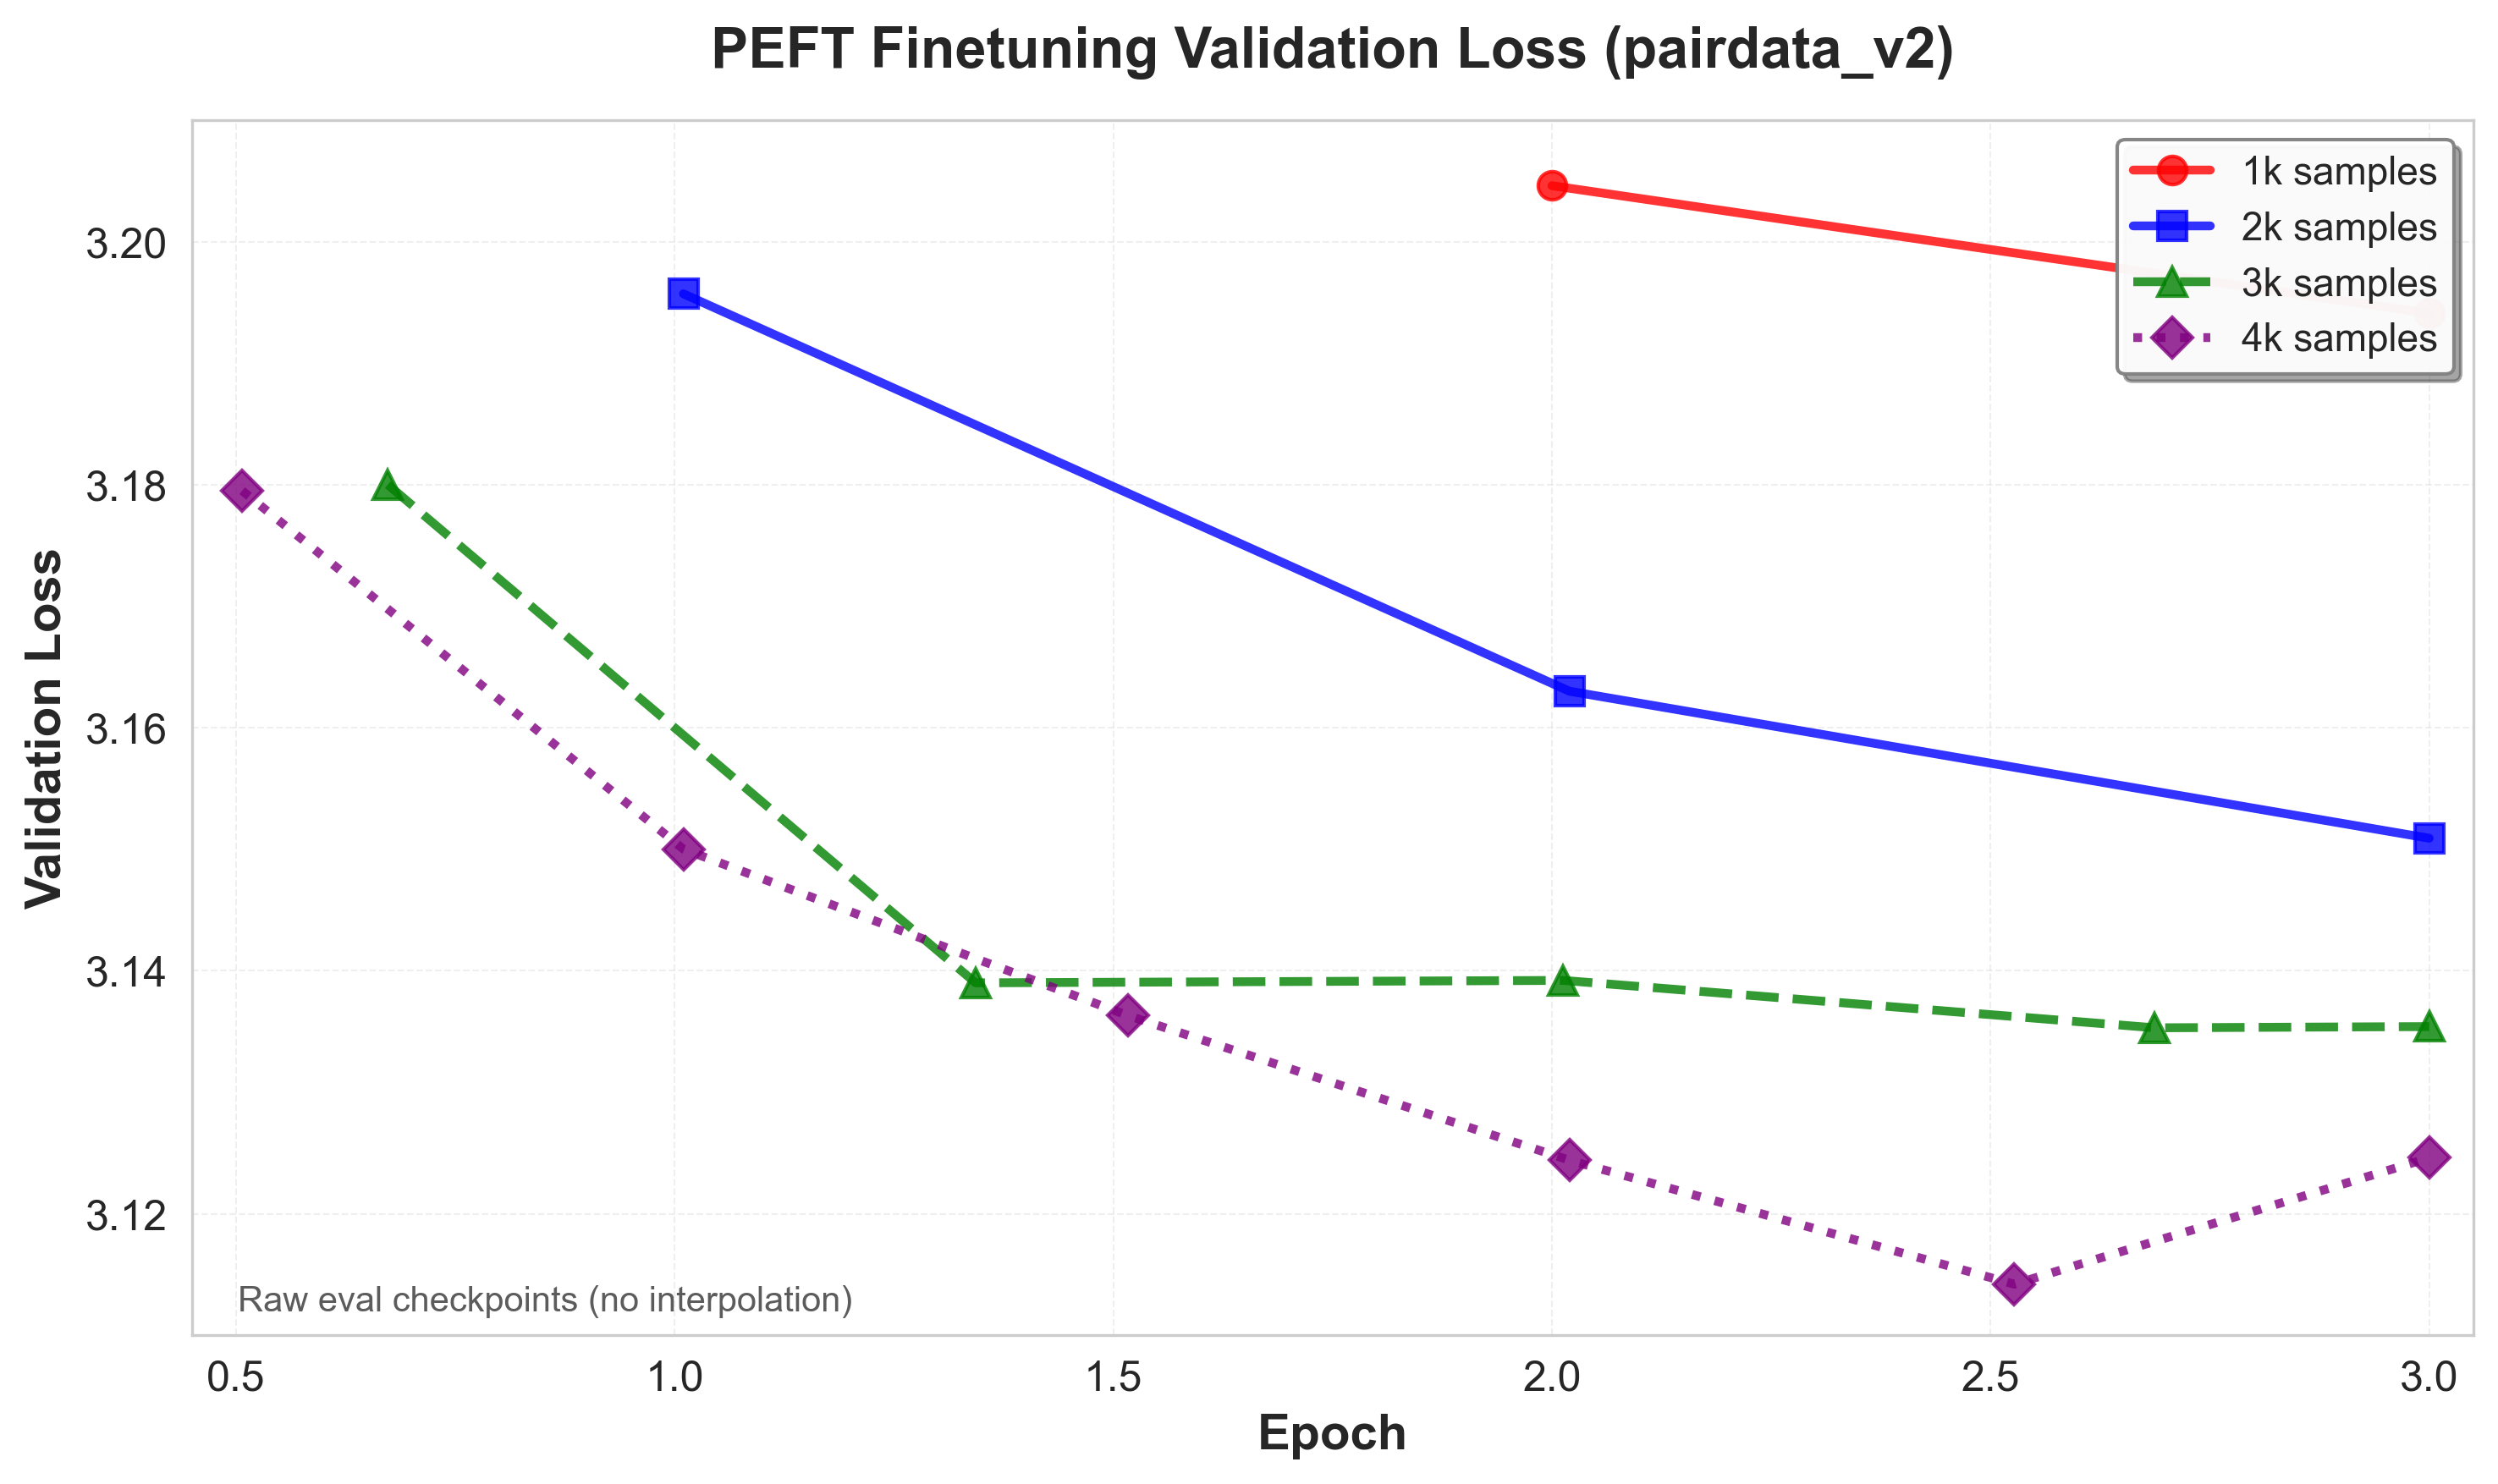
\includegraphics[width=0.55\columnwidth]{figures_vlm/11_s4_validation_loss_pairdata_v2.png}
\caption{Validation loss trajectories in S.4 progressive retraining on pairdata\_v2.
Curves follow the same visual style as Figure~9 for direct comparison.
Points are plotted at raw evaluation checkpoints from each run (no interpolation);
therefore the first 1\,k point appears at epoch~2 because eval\_steps was 100.
The 4\,k run reaches the lowest value at epoch~2 (3.124) and then changes only marginally at epoch~3 (3.125).}
\label{fig:s4_val_loss}
\end{figure}

\subsubsection*{Observations}

A notable pattern emerges across scales: teacher-forcing token accuracy
undergoes a sharp transition between epoch~1 and epoch~2.
For the 2\,k model, accuracy rises from $89.3$\,\% to $98.5$\,\% over a
single epoch, while eval loss decreases by only $0.033$ nats.
This dissociation suggests that the model converges on the \emph{ordering}
of tokens (argmax identity) much faster than it converges on the full
log-probability distribution, a consequence of the softmax sharpening
characteristic of fine-tuning at low learning rates.

Comparing all four scales reveals a consistent pattern of diminishing
returns (Table~\ref{tab:s4_progressive}):
\begin{itemize}
  \item $1\text{k} \to 2\text{k}$: eval loss $3.194 \to 3.151$
        ($\Delta = {-}0.043$\,nats), token acc.\ $90.1 \to 98.7$\,\%
        ($\Delta = {+}8.6$\,pp)
  \item $2\text{k} \to 3\text{k}$: eval loss $3.151 \to 3.135$
        ($\Delta = {-}0.016$\,nats), token acc.\ $98.7 \to 99.0$\,\%
        ($\Delta = {+}0.3$\,pp)
  \item $3\text{k} \to 4\text{k}$: eval loss $3.135 \to 3.125$
        ($\Delta = {-}0.010$\,nats), token acc.\ $99.0 \to 99.2$\,\%
        ($\Delta = {+}0.2$\,pp)
\end{itemize}
The largest gains concentrate in the first doubling ($1\text{k} \to 2\text{k}$);
beyond 2\,k the per-step improvement falls below $0.020$ nats per thousand
samples, indicating that the LoRA adapter is approaching its capacity
under the current rank~32 configuration.
A secondary observation concerns the 4\,k epoch-level profile: eval loss
reaches its minimum at epoch~2 ($3.124$) and rises marginally at
epoch~3 ($3.125$), suggesting the onset of overfitting at the largest
scale, absent in the 1\,k--3\,k runs.
This pattern is visible in Figure~\ref{fig:s4_val_loss}, where the
4\,k trajectory flattens after epoch~2 while lower-scale curves show
larger between-epoch movement.

%%--------------------------------------------------------------------
\subsection*{S.6 Semantic Similarity on Denoised Test Set}
%%--------------------------------------------------------------------

\begin{sloppypar}
Table~\ref{tab:s6_results} reports cosine similarity between model predictions
and denoised pairdata-v2 ground truth for all four training scales
($n=800$ test set, 2{,}048-dimensional composite embedding evaluator:
\nolinkurl{hotchpotch/static-embedding-japanese}~$\oplus$
\nolinkurl{intfloat/multilingual-e5-large}; see method description below).
The 2k model reaches the \textit{Good} tier majority under pairdata-v2
thresholds (Excellent$\geq$0.85, Good$\geq$0.70, Acceptable$\geq$0.55).
\end{sloppypar}

\begin{table}[h]
\centering
\caption{Cosine similarity on denoised test set (v0.7.2, pairdata-v2, $n=800$,
         2{,}048-dim composite evaluator).
         Thresholds: Excellent$\geq$0.85, Good$\geq$0.70,
         Acceptable$\geq$0.55, Poor$\geq$0.40, Very~Poor$<$0.40.}
\label{tab:s6_results}
\setlength{\tabcolsep}{4pt}
\small
\begin{tabular}{lrrrrr}
\toprule
Scale & $\bar{\rho}$ & $\sigma$ & Median & Good$+$ (\%) & V.\,Poor (\%) \\
\midrule
1k & 0.6725 & 0.0706 & 0.6749 & 37.8 & 0.4 \\
2k & 0.6950 & 0.0824 & 0.7053 & 53.1 & 0.4 \\
3k & 0.6767 & 0.0751 & 0.6799 & 37.8 & 0.4 \\
4k & 0.6749 & 0.0742 & 0.6803 & 38.4 & 0.4 \\
\bottomrule
\end{tabular}
\end{table}

Key findings: (i)~scaling from 1k to 2k yields $+3.3\%$ mean improvement
($0.6725\to0.6950$) and pushes the median above the Good threshold
($0.7053$); (ii)~3k and 4k both regress toward 1k levels
($\bar{\rho}_{3k}=0.6767$, $\bar{\rho}_{4k}=0.6749$), indicating
overfitting beyond 2k; (iii)~the Good-tier majority is achieved only
at 2k ($53.1\%$ Good$+$Excellent), while all other scales plateau near
$37$--$38\%$; (iv)~the Very~Poor rate is uniformly negligible
($\approx$0.4\%) across all scales, reflecting the substantially higher
discriminative power of the 2{,}048-dim composite evaluator compared
with the 384-dim single-model baseline.

Figure~\ref{fig:s6_similarity} shows mean and median cosine similarity
with $\pm\sigma$ error bars across training scales, overlaid with
384-dim MiniLM baseline values (red dashed), confirming
the consistent gain from the composite evaluator and the
inverted-U pattern peaking at 2k.

\begin{figure}[H]
\centering
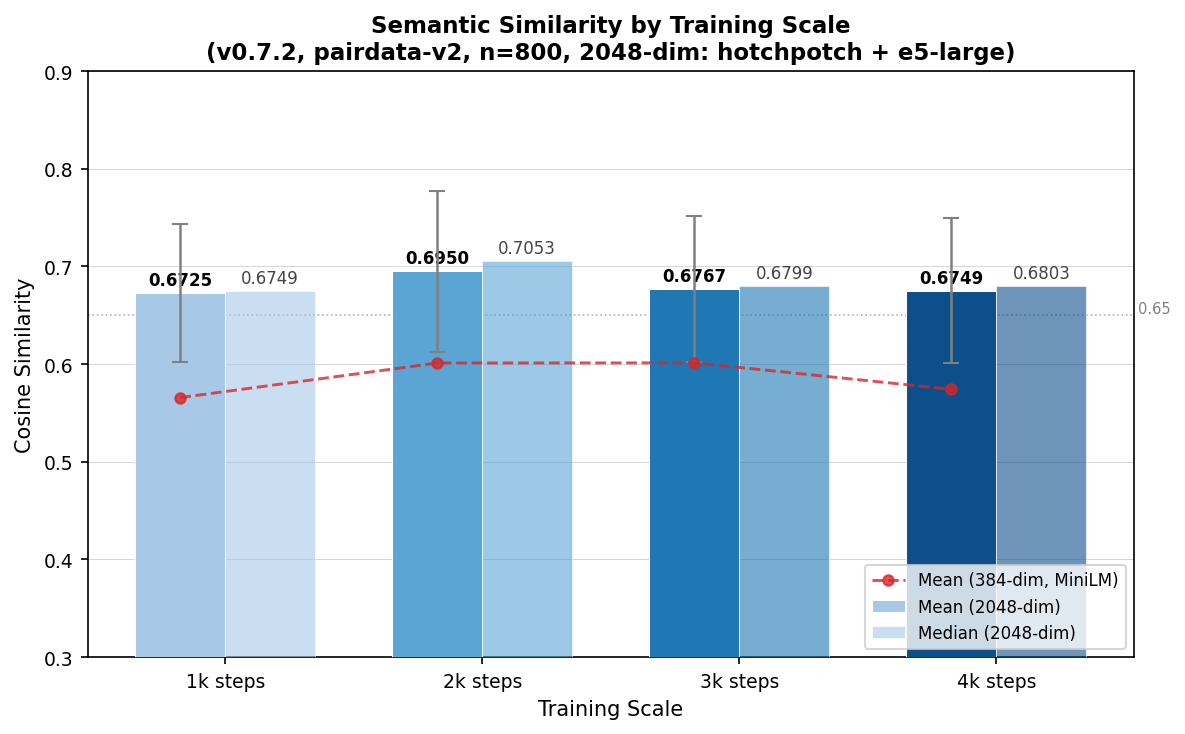
\includegraphics[width=0.44\textwidth]{figures_vlm/12_v072_similarity_by_scale.png}
\caption{Mean and median cosine similarity by training scale
(v0.7.2, pairdata-v2, $n=800$, 2{,}048-dim composite evaluator).
Error bars: $\pm\sigma$. Red dashed: 384-dim MiniLM baseline.
Peak at 2k; 3k and 4k regress toward 1k levels.}
\label{fig:s6_similarity}
\end{figure}

\begin{figure}[H]
\centering
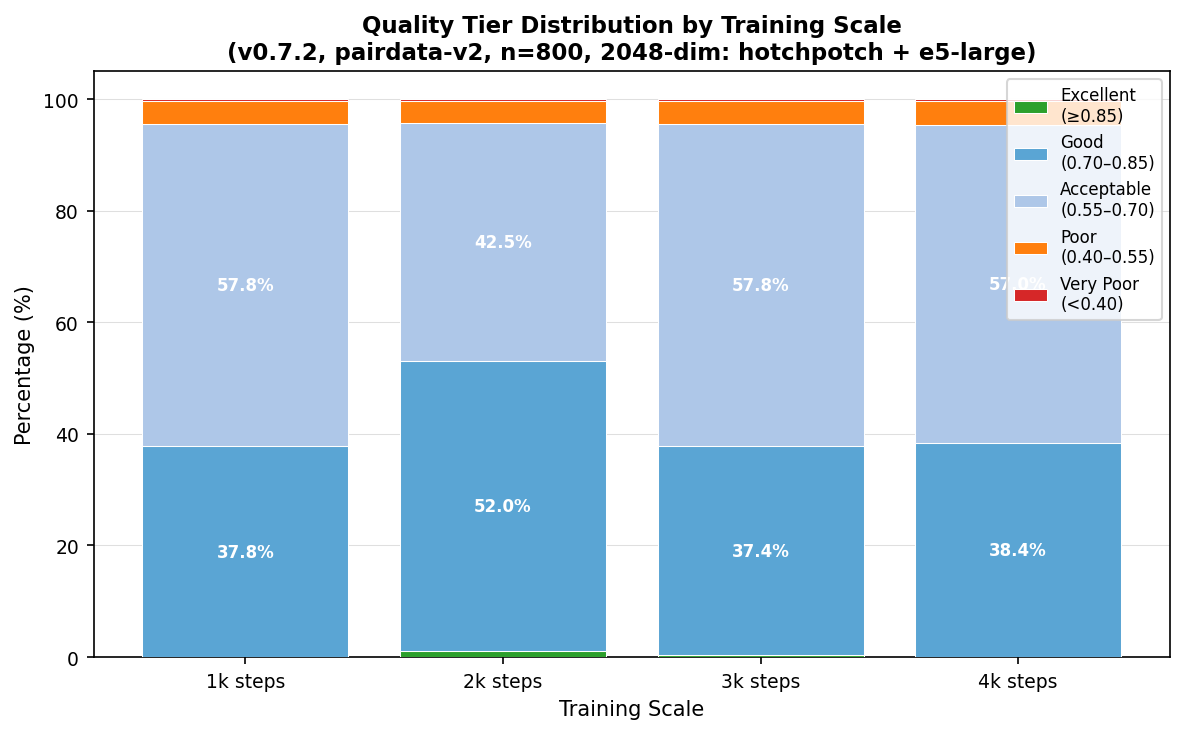
\includegraphics[width=0.44\textwidth]{figures_vlm/13_v072_tier_distribution.png}
\caption{Quality-tier distribution by training scale (v0.7.2, pairdata-v2,
2{,}048-dim composite evaluator).
Stacked bars (100\% basis) show share of each tier across $n=800$ samples.
Good tier peaks at 2k ($52.0\%$); Very~Poor is negligible ($<$0.4\%)
across all scales.}
\label{fig:s6_tier}
\end{figure}

\begin{figure}[H]
\centering
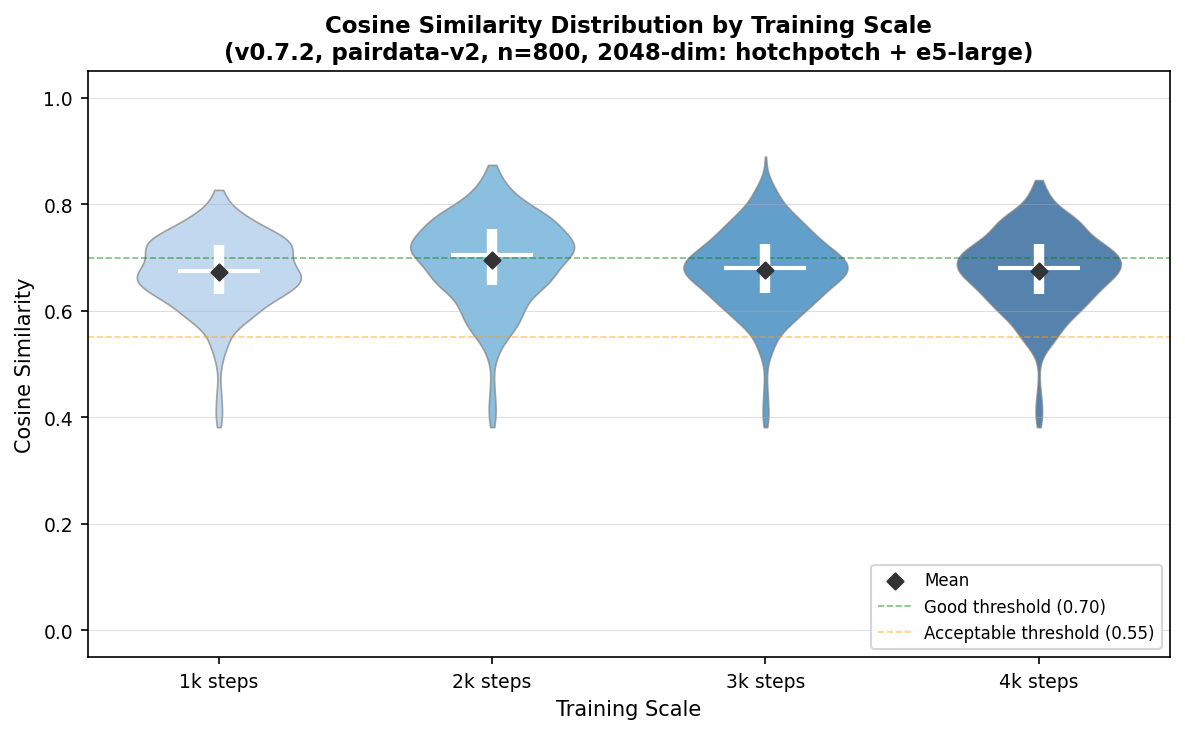
\includegraphics[width=0.44\textwidth]{figures_vlm/14_v072_cosine_violin.png}
\caption{Cosine similarity distributions as violin plots (v0.7.2, pairdata-v2,
2{,}048-dim composite evaluator).
Diamond: mean; white dot: median; thick bar: IQR.
The 2k distribution is visibly shifted rightward; all scales show
negligible density below the Acceptable threshold ($\rho<0.55$).}
\label{fig:s6_violin}
\end{figure}

\medskip
\noindent\textbf{Model selection.}
Based on the denoised pairdata-v2 evaluation with the 2{,}048-dimensional
composite evaluator, the \textbf{2k model} is selected as the recommended
deployment configuration.
It achieves the peak mean cosine similarity ($\bar{\rho}_{2k}=0.6950$,
Table~\ref{tab:s6_results}), the highest median ($0.7053$, above the Good
threshold), and the highest Good-tier rate ($53.1\%$) among all four scales.
The 3k and 4k models both regress: $\bar{\rho}_{3k}=0.6767$
($-2.6\%$ vs.\ 2k) and $\bar{\rho}_{4k}=0.6749$ ($-2.9\%$ vs.\ 2k),
consistent with overfitting beyond 2k training steps.
The Very~Poor rate is uniformly negligible ($\approx$0.4\%) across all
scales, reflecting the substantially higher discriminative power of the
2{,}048-dim composite evaluator.
This recommendation differs from the pairdata-v1 finding (main body,
Section~\ref{sec:results}), where the 3k model achieved peak performance
($\bar{\rho}_{3k}=0.6909$); the discrepancy suggests that the denoised
pairdata-v2 annotations are more sensitive to early-stage overfitting,
making 2k the optimal scale under this stricter evaluation.

%%--------------------------------------------------------------------
\subsubsection*{Extended Evaluation: 2\,048-Dimensional Composite Embeddings}

To improve semantic fidelity beyond the single-model 384-dimensional baseline,
we design a composite embedding that combines two complementary Japanese-capable
sentence encoders:
\begin{sloppypar}
\begin{itemize}[noitemsep, topsep=2pt]
  \item $\mathcal{M}_1$:~\nolinkurl{hotchpotch/static-embedding-japanese}
    ---1\,024 dimensions, static \texttt{EmbeddingBag} model
    trained on Japanese corpora; inference is entirely CPU-native.
  \item $\mathcal{M}_2$:~\nolinkurl{intfloat/multilingual-e5-large}
    ---1\,024 dimensions, Transformer encoder supporting 100+ languages;
    for symmetric STS tasks the prefix \texttt{"query:~"} is prepended
    to \emph{both} ground-truth and prediction texts.
\end{itemize}
\end{sloppypar}

\noindent
For each text $t$, both encoders independently produce $L_2$-normalised embeddings:
\begin{equation}
  \mathbf{e}_1(t) =
    \frac{f_{\mathcal{M}_1}(t)}{\bigl\|f_{\mathcal{M}_1}(t)\bigr\|_2}
    \;\in\;\mathbb{R}^{1024},
  \qquad
  \mathbf{e}_2(t) =
    \frac{f_{\mathcal{M}_2}(\texttt{``query:\ ''}\!\parallel\!t)}
         {\bigl\|f_{\mathcal{M}_2}(\texttt{``query:\ ''}\!\parallel\!t)\bigr\|_2}
    \;\in\;\mathbb{R}^{1024}.
  \label{eq:e1e2}
\end{equation}
The two vectors are concatenated along the feature axis and re-normalised
to form the 2\,048-dimensional composite representation:
\begin{equation}
  \mathbf{e}(t) =
    \frac{\bigl[\mathbf{e}_1(t)\;;\;\mathbf{e}_2(t)\bigr]}
         {\bigl\|\bigl[\mathbf{e}_1(t)\;;\;\mathbf{e}_2(t)\bigr]\bigr\|_2}
    \;\in\;\mathbb{R}^{2048}.
  \label{eq:concat}
\end{equation}
Since $\|\mathbf{e}_1\|_2 = \|\mathbf{e}_2\|_2 = 1$, the concatenated
norm equals $\sqrt{2}$, and the cosine similarity between ground-truth
$t^{\mathrm{gt}}$ and prediction $t^{\mathrm{pred}}$ simplifies to
\begin{equation}
  \rho_{2048}
    \;=\; \mathbf{e}(t^{\mathrm{gt}})\cdot\mathbf{e}(t^{\mathrm{pred}})
    \;=\; \frac{
      \mathbf{e}_1^{\mathrm{gt}}\cdot\mathbf{e}_1^{\mathrm{pred}}
      + \mathbf{e}_2^{\mathrm{gt}}\cdot\mathbf{e}_2^{\mathrm{pred}}
    }{2}
    \;=\; \frac{\rho_1 + \rho_2}{2},
  \label{eq:rho2048}
\end{equation}
i.e.\ the arithmetic mean of the two per-model cosine similarities.
$\mathcal{M}_1$ contributes Japanese lexical specificity
via its static embedding lookup, while $\mathcal{M}_2$ provides
broader multilingual semantic coverage through its Transformer encoder.
The combined evaluator operates entirely on CPU without GPU resources.

%%--------------------------------------------------------------------
\subsection*{S.7 Quality Guard Recalibration (v0.7.3 / v0.7.5)}
%%--------------------------------------------------------------------

\noindent
The Quality Guard thresholds ($\theta_{\text{low}}$, $\theta_{\text{high}}$)
calibrated for pairdata-v1 (v0.6.3: $\theta_{\text{low}}=98$,
$\theta_{\text{high}}=202$) were found to be inappropriate for
pairdata-v2 model outputs.
Denoised training data produces shorter, more concise predictions
compared to the noisier pairdata-v1 outputs.
This section reports the recalibration procedure (introduced in v0.7.3 with
the 3k model) and the full pipeline results for \textbf{v0.7.5}, which
adopts the \textbf{2k model} as identified optimal by the
2{,}048-dimensional composite embedding evaluation in Section~S.6.

\medskip
\noindent\textbf{Recalibration procedure.}
Token counts were computed for all $n=800$ predictions using the
approximate CJK+ASCII tokeniser.
For the 3k model (v0.7.3): mean~103 tokens, $\sigma$~29, $p_5=60$, max~196;
applying the old $\theta_{\text{low}}=98$ would reject $\approx$50\,\% of valid
predictions.
For the 2k model (v0.7.5): mean~112 tokens, $\sigma$~22, $p_5=87$, max~181;
the distribution is slightly longer and more compact.
In both cases all predictions with fewer than 30 tokens are
file-not-found error strings with no diagnostic content.
Thresholds were therefore set to:
\[
  \theta_{\text{low}} = 30 \quad (\text{was } 98),
  \qquad
  \theta_{\text{high}} = 200 \quad (\text{was } 202).
\]
Figure~\ref{fig:s7_token} compares the token count histograms of the
3k model (v0.7.3, left) and 2k model (v0.7.5, right) with both the old
and recalibrated $\theta_{\text{low}}$ overlaid.
The shaded band (30--98) indicates the region reclaimed as valid.

\begin{figure}[H]
\centering
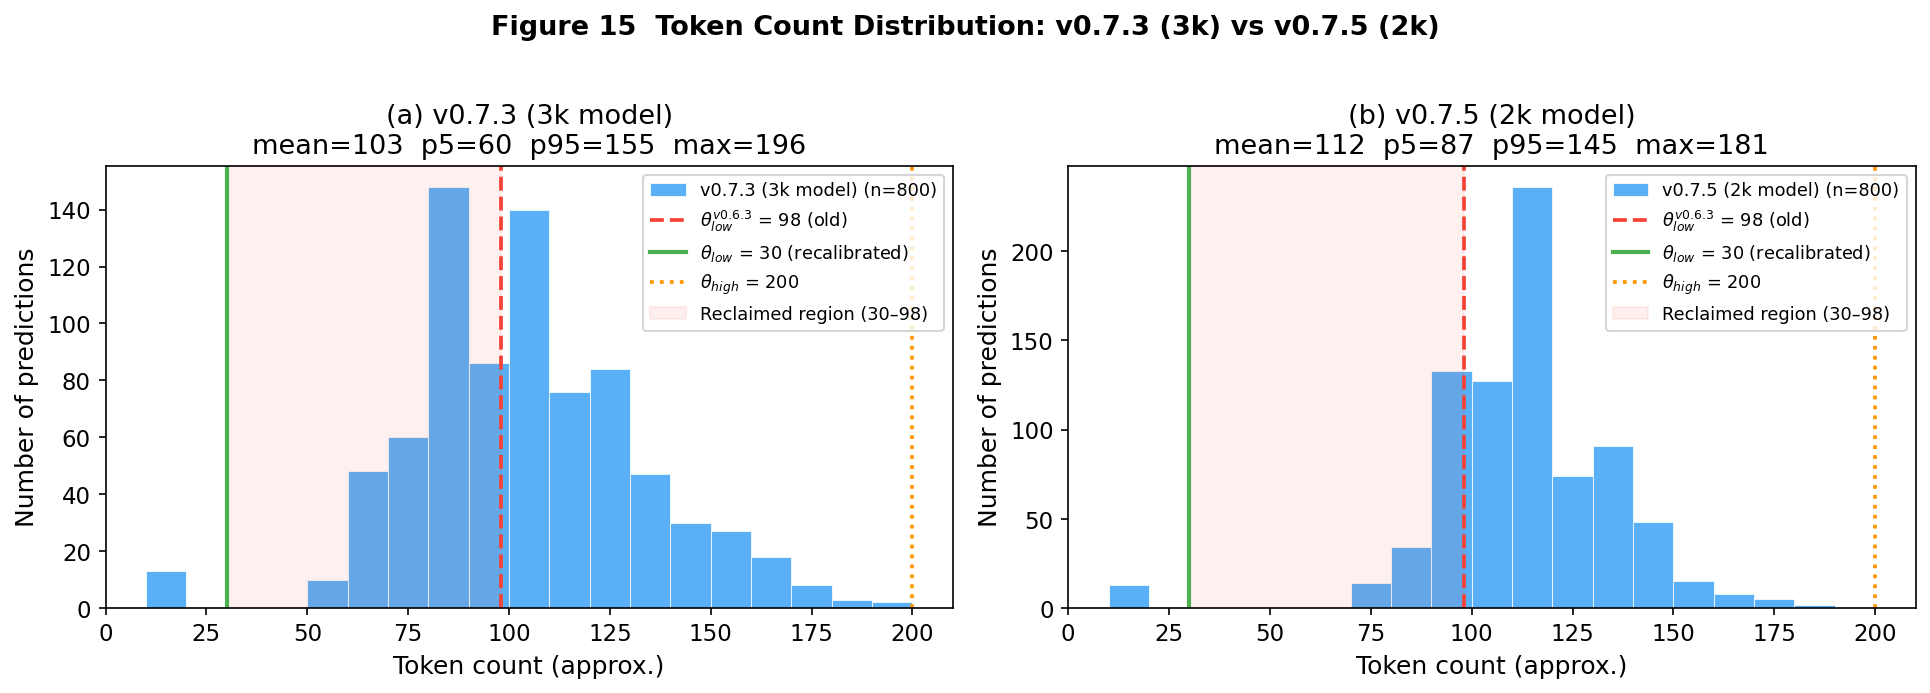
\includegraphics[width=0.95\textwidth]{figures_vlm/15_v073_token_distribution.png}
\caption{Token count distributions: v0.7.3 3k model (left) and v0.7.5 2k model (right).
         Dashed red: old $\theta_{\text{low}}^{v0.6.3}=98$;
         solid green: recalibrated $\theta_{\text{low}}=30$;
         dotted: $\theta_{\text{high}}=200$.
         The shaded band shows the reclaimed valid region.
         The 2k model produces slightly longer outputs (mean~112 vs.~103 tokens)
         with lower variance ($\sigma$~22 vs.~29).}
\label{fig:s7_token}
\end{figure}

\medskip
\noindent\textbf{v0.7.5 pipeline results ($n=800$, 2k model).}
Running the full Quality Guard + Priority Scoring pipeline with
recalibrated thresholds on the 2k model inference results yields the
same PASS rate as v0.7.3 (3k model), confirming threshold stability:

\begin{table}[H]
\centering
\caption{Quality Guard recalibration results: v0.7.3 (3k model) and v0.7.5
         (2k model), pairdata-v2, $n=800$.
         Pipeline: rule-based guard ($\theta_{\text{low}}=30$,
         $\theta_{\text{high}}=200$) + keyword structuring + priority scoring.}
\label{tab:s7_guard}
\small
\begin{tabular}{lrrrr}
\toprule
 & \multicolumn{2}{c}{v0.7.3 (3k)} & \multicolumn{2}{c}{v0.7.5 (2k)} \\
\cmidrule(lr){2-3}\cmidrule(lr){4-5}
Verdict / Reason & Count & Rate (\%) & Count & Rate (\%) \\
\midrule
PASS --- High Quality            & 787 & 98.4 & 787 & 98.4 \\
FAIL --- Too short / Error output &  13 &  1.6 &  13 &  1.6 \\
\midrule
Total                             & 800 & 100.0 & 800 & 100.0 \\
\bottomrule
\end{tabular}
\end{table}

\noindent
The rejection rate is identical for both models (1.6\,\%),
confirming that the recalibrated thresholds generalise across pairdata-v2
model variants.
All 13 rejected outputs are file-not-found error strings produced
when the image loader could not locate a file.

\medskip
\noindent\textbf{Discussion.}
The high PASS rate of 98.4\,\% reflects a qualitative improvement
in the inference outputs generated from pairdata~v2.
Compared with pairdata~v1, the fine-tuning corpus for v2 was
curated to remove noise content that fell outside the intended
scope of structural-damage recognition---such as scene-level
descriptions unrelated to member condition or administrative
metadata copied from inspection templates.
By filtering out these out-of-scope patterns during training-data
construction, the resulting models produce outputs that are
structurally valid and damage-focused, thereby passing the
token-range and format checks of the Quality Guard at a markedly
higher rate.

\medskip
\noindent\textbf{Priority distribution (v0.7.5, 2k model).}
Among the 787 PASS predictions, priority scoring yields:
Level~3 (Planned maintenance): 30 images (3.8\,\%);
Level~4 (Priority repair): 755 images (95.9\,\%);
Level~5 (Immediate repair): 2 images (0.3\,\%).
For comparison, the v0.7.3 3k model yielded:
Level~3: 21 (2.7\,\%), Level~4: 651 (82.7\,\%), Level~5: 115 (14.6\,\%).
Both models resolve the Level~3 saturation of v0.6.3, but their severity
profiles differ: the 2k model concentrates predictions at Level~4
(95.9\,\%), whereas the 3k model distributes more mass at Level~5
(14.6\,\%).
This difference reflects the 2k model generating slightly more moderate-severity
vocabulary (\textit{mean token count~112 vs.~103}), which the keyword
scorer maps to Level~4 rather than Level~5
(Figure~\ref{fig:s7_priority}).

\begin{figure}[H]
\centering
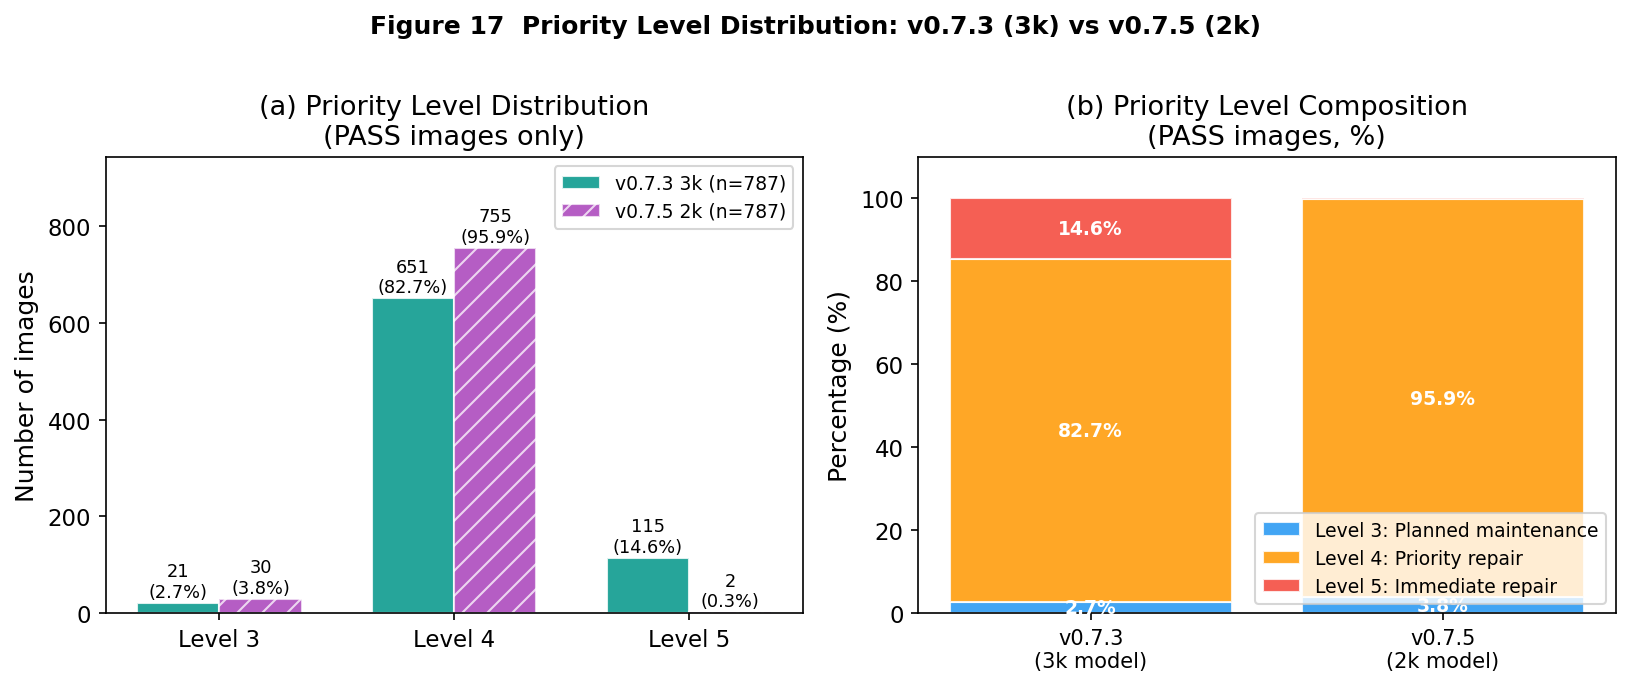
\includegraphics[width=0.88\textwidth]{figures_vlm/17_v073_priority_distribution.png}
\caption{Priority level distribution comparison: v0.7.3 3k model and v0.7.5 2k model
         (PASS predictions, $n=787$ each).
         Left: grouped bar chart (absolute counts); Right: stacked percentage view.
         Both models resolve the Level~3 saturation of v0.6.3.
         The 2k model (v0.7.5) concentrates at Level~4 (95.9\,\%),
         while the 3k model (v0.7.3) distributes more mass at Level~5 (14.6\,\%).}
\label{fig:s7_priority}
\end{figure}

\begin{figure}[H]
\centering
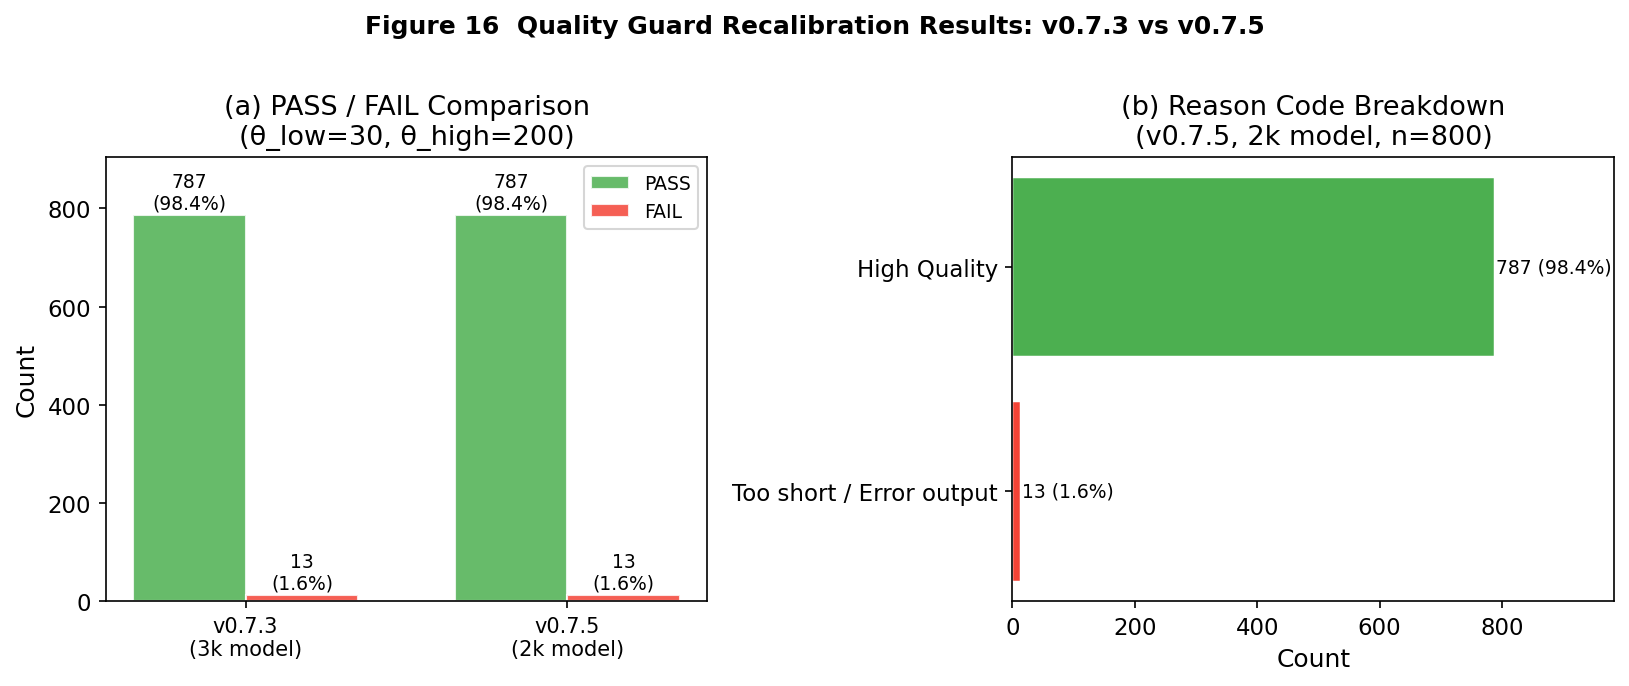
\includegraphics[width=0.85\textwidth]{figures_vlm/16_v073_guard_breakdown.png}
\caption{Quality Guard recalibration results (v0.7.3 vs.\, v0.7.5, $n=800$).
         Left: PASS/FAIL verdict comparison (both 98.4\,\% PASS);
         Right: reason code breakdown for v0.7.5 (2k model).}
\label{fig:s7_guard}
\end{figure}

% ── S.7.1 Structural Member and Damage Type Comparison ─────────────
\subsection*{S.7.1\quad Structural Member and Damage Type: pairdata v1 vs.\ v2}

To clarify the behavioral change introduced by pairdata~v2 (v0.7.3),
we replicate the structural member and damage-type analysis of
Figure~10 in the main body and apply it to both pipeline versions
(Figure~\ref{fig:s71_member_damage}).

\begin{figure}[H]
\centering
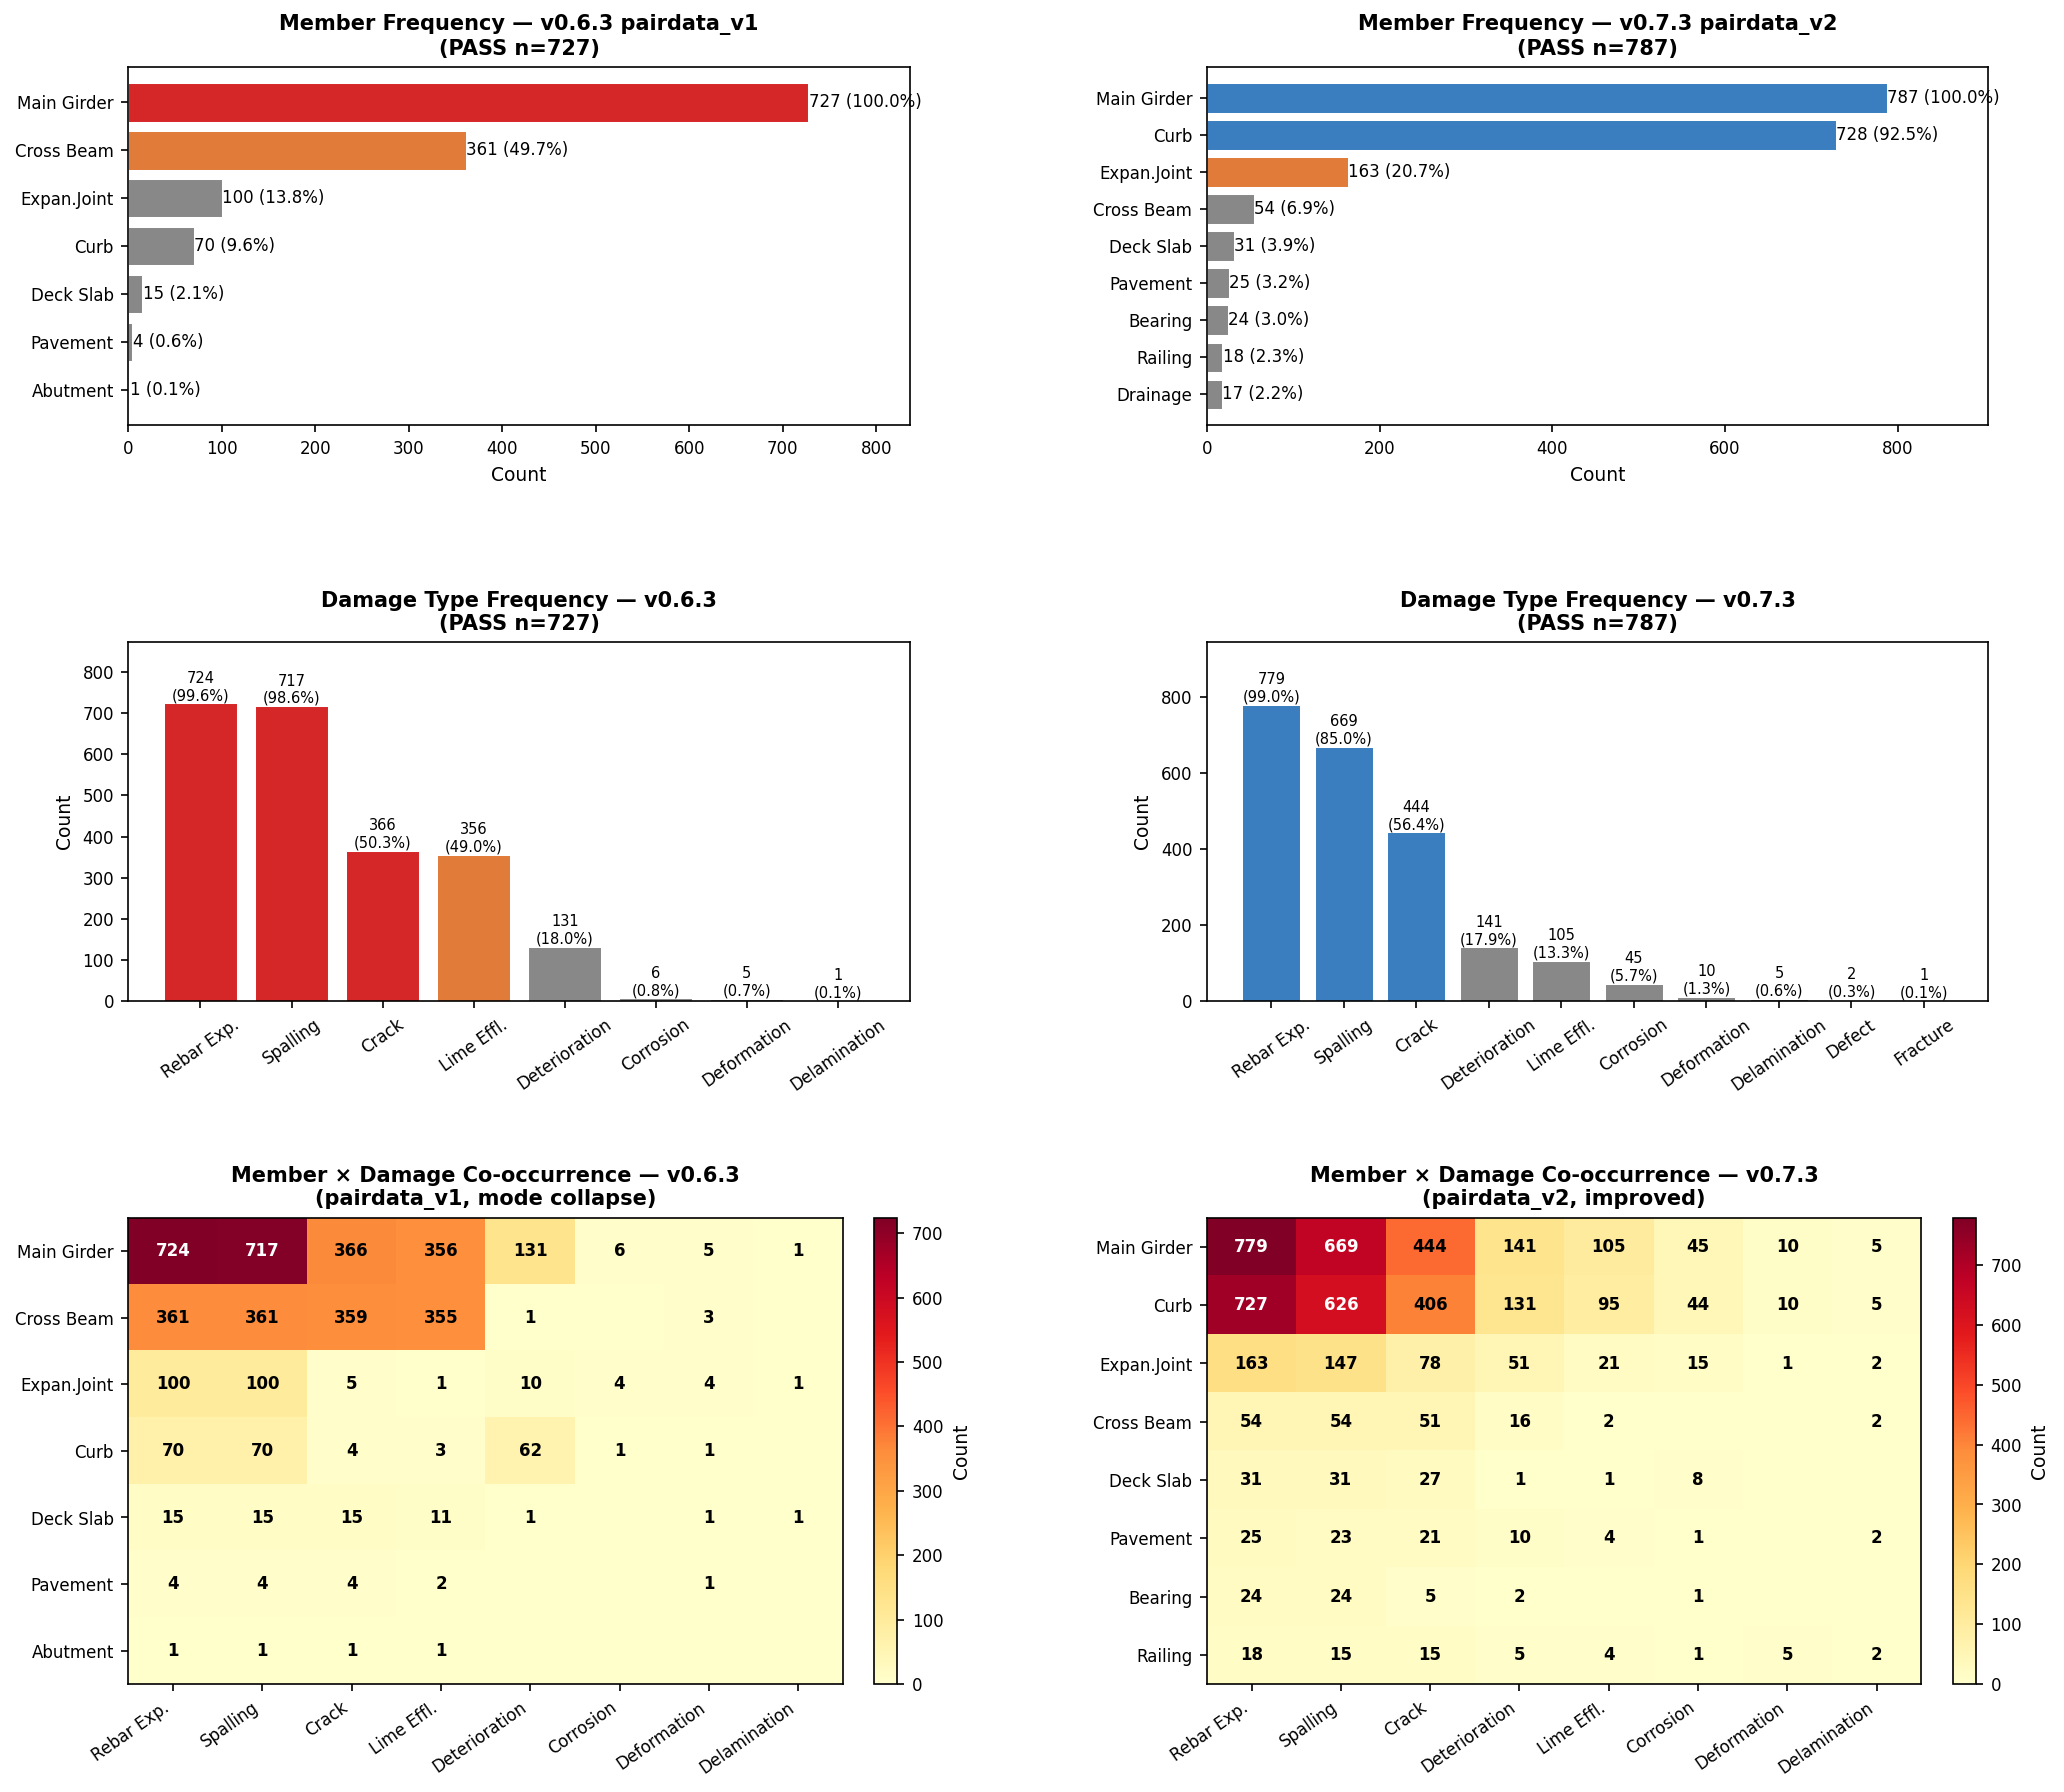
\includegraphics[width=0.9\textwidth]{figures_vlm/18_member_damage_comparison.png}
\caption{Structural member and damage type analysis for PASS samples:
         \textit{left column} v0.6.3 pairdata\_v1 ($n=727$),
         \textit{right column} v0.7.3 pairdata\_v2 ($n=787$).
         \textit{Top}: member mention frequency;
         \textit{Middle}: damage type frequency;
         \textit{Bottom}: member $\times$ damage co-occurrence heatmap.}
\label{fig:s71_member_damage}
\end{figure}

\paragraph{Member distribution.}
Both versions share Main Girder dominance (100\,\%), but the
secondary-member pattern differs markedly.
In v0.6.3, Cross Beam appears as secondary at 49.7\,\%, reflecting
a generalized bridge-body description.
In v0.7.3, Curb rises to 92.5\,\%, indicating that the 3k
model trained on pairdata\_v2 now explicitly localizes rebar-exposure
damage to the overhang and parapet region.
This change is expected: pairdata\_v2 was curated to include diverse
rebar-exposure examples captured at curb and fascia locations,
prompting the model to identify that structural zone.

\paragraph{Damage type distribution.}
Rebar Exposure remains the dominant keyword in both versions
(v0.6.3: 99.6\,\%; v0.7.3: 99.0\,\%).
However, the co-occurrence heatmap reveals a structural shift:
v0.6.3 assigns nearly identical counts to Main Girder $\times$
Rebar Exposure (724) and Main Girder $\times$ Spalling (717),
reflecting the mode-collapsed vocabulary that caused scoring saturation.
In v0.7.3, Crack mentions increase to 56.4\,\% (vs.\ 50.3\,\%),
and Lime Efflorescence drops to 13.3\,\% (vs.\ 49.0\,\%),
suggesting a more focused and contextually appropriate description
of rebar-exposure-related deterioration.

\paragraph{Discussion: bias suppression through noise removal.}
The distributional shifts observed above are a direct consequence of
the noise-removal strategy applied during pairdata~v2 construction.
In pairdata~v1, the fine-tuning corpus contained out-of-scope
descriptions: generic bridge overviews, administrative metadata
transcribed from inspection templates, and multi-member narratives
that enumerated components regardless of whether they appeared
in the target image.
The model trained on this data acquired a stereotyped co-occurrence
pattern---routinely pairing Main Girder with Cross Beam, Rebar
Exposure, and Spalling as a fixed vocabulary template, independent
of actual image content.
This is evidenced by the nearly equal counts of Main Girder $\times$
Rebar Exposure (724) and Main Girder $\times$ Spalling (717) in
v0.6.3, and by the high Lime Efflorescence rate (49.0\,\%) despite
the test set consisting primarily of rebar-exposure images where
lime efflorescence is not the dominant deterioration form.

In pairdata~v2, out-of-scope content was removed so that each
training example describes only the damage visible within the image
frame.
The resulting model exhibits reduced output bias: the near-identical
Rebar Exposure--Spalling coupling breaks down (Spalling drops from
98.6\,\% to 85.0\,\%), Lime Efflorescence falls to 13.3\,\%,
and the secondary member shifts from the stereotyped Cross Beam
to Curb---the structural zone where rebar-exposure damage is
physically concentrated in the test images.
Together, these changes confirm that noise removal in the
training corpus is an effective mechanism for suppressing
hallucinated co-occurrence patterns and aligning model output
with image-specific damage evidence.

\paragraph{Model scale comparison: v0.7.3 (3k) vs.\ v0.7.5 (2k).}
To assess whether reducing the training duration from 3k to 2k steps
affects structural member and damage-type vocabulary, we apply the
same analysis to v0.7.5 (Figure~\ref{fig:s71_member_damage_v075}).
Main Girder dominance (100\,\%) and Curb co-occurrence (94.7\,\%)
are preserved across both scales, confirming that the spatial
localization improvement introduced by pairdata~v2 is robust to
model size.
However, a notable divergence appears in the Cross Beam mention rate:
the 2k model (v0.7.5) includes Cross Beam in 98.3\,\% of predictions,
compared to only 6.9\,\% in the 3k model (v0.7.3).
This elevated cross-beam co-occurrence---recalling the pattern
observed in v0.6.3 (49.7\,\%)---suggests that shorter training
on pairdata~v2 retains a partial template pairing Main Girder with
Cross Beam as a structural header, even when the target damage is
localized to the curb zone.
Despite this vocabulary difference, the co-occurrence heatmaps
show no systematic shift in damage-member coupling between the two
scales, and overall priority scoring behavior (see S.7.2) remains
consistent, confirming that pairdata~v2 quality is the primary
driver of scoring improvement rather than the number of training steps.

\begin{figure}[H]
\centering
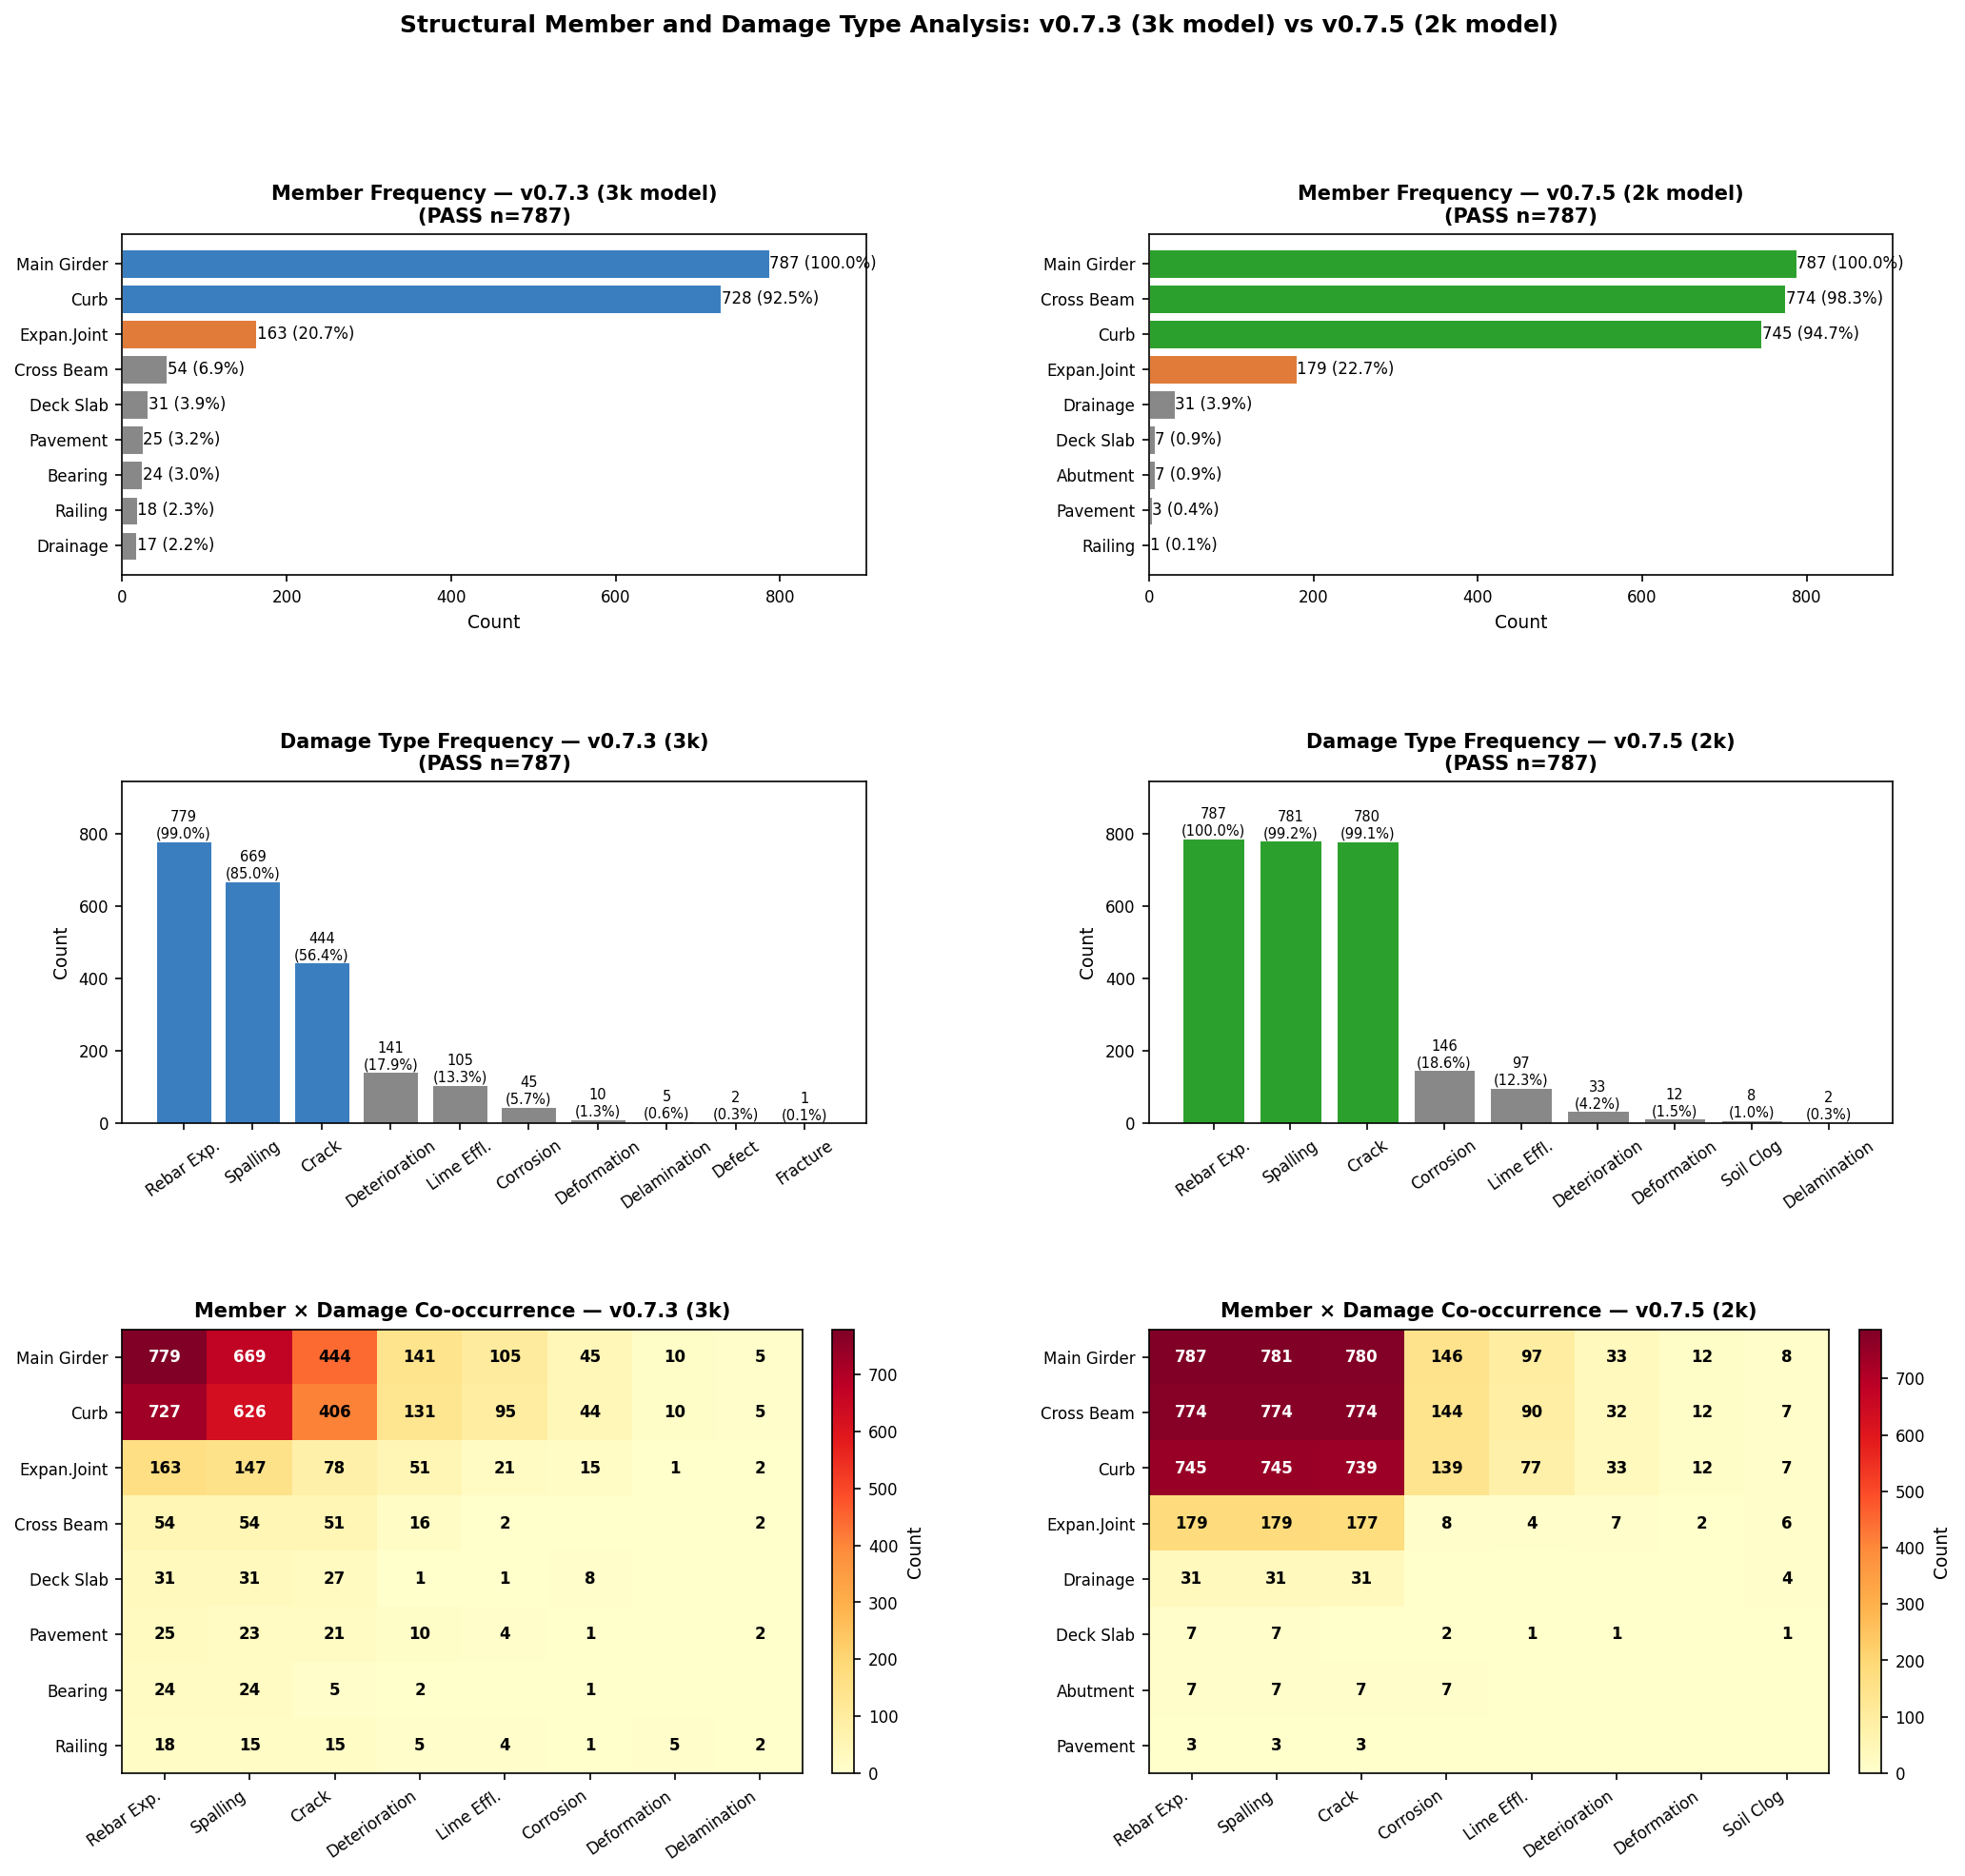
\includegraphics[width=0.9\textwidth]{figures_vlm/19_member_damage_v073_v075.png}
\caption{Structural member and damage type analysis: v0.7.3 (3k model) vs.\
         v0.7.5 (2k model) (PASS samples, $n=787$ each).
         \textit{Left column}: v0.7.3 (3k); \textit{Right column}: v0.7.5 (2k).
         \textit{Top}: member mention frequency;
         \textit{Middle}: damage type frequency;
         \textit{Bottom}: member $\times$ damage co-occurrence heatmap.
         Both scales maintain Curb localization ($\geq92.5\,\%$);
         the 2k model additionally shows elevated Cross Beam
         co-occurrence (98.3\,\% vs.\ 6.9\,\%), suggesting partial
         retention of a generalized description template.}
\label{fig:s71_member_damage_v075}
\end{figure}

% ── S.7.2 Priority Score Distribution ─────────────────────────────────
\subsection*{S.7.2\quad Priority Score Distribution}

Figure~\ref{fig:s72_violin} presents the continuous priority-score
distributions for three pipeline versions using violin plots and
stacked level-composition bars.

\begin{figure}[H]
\centering
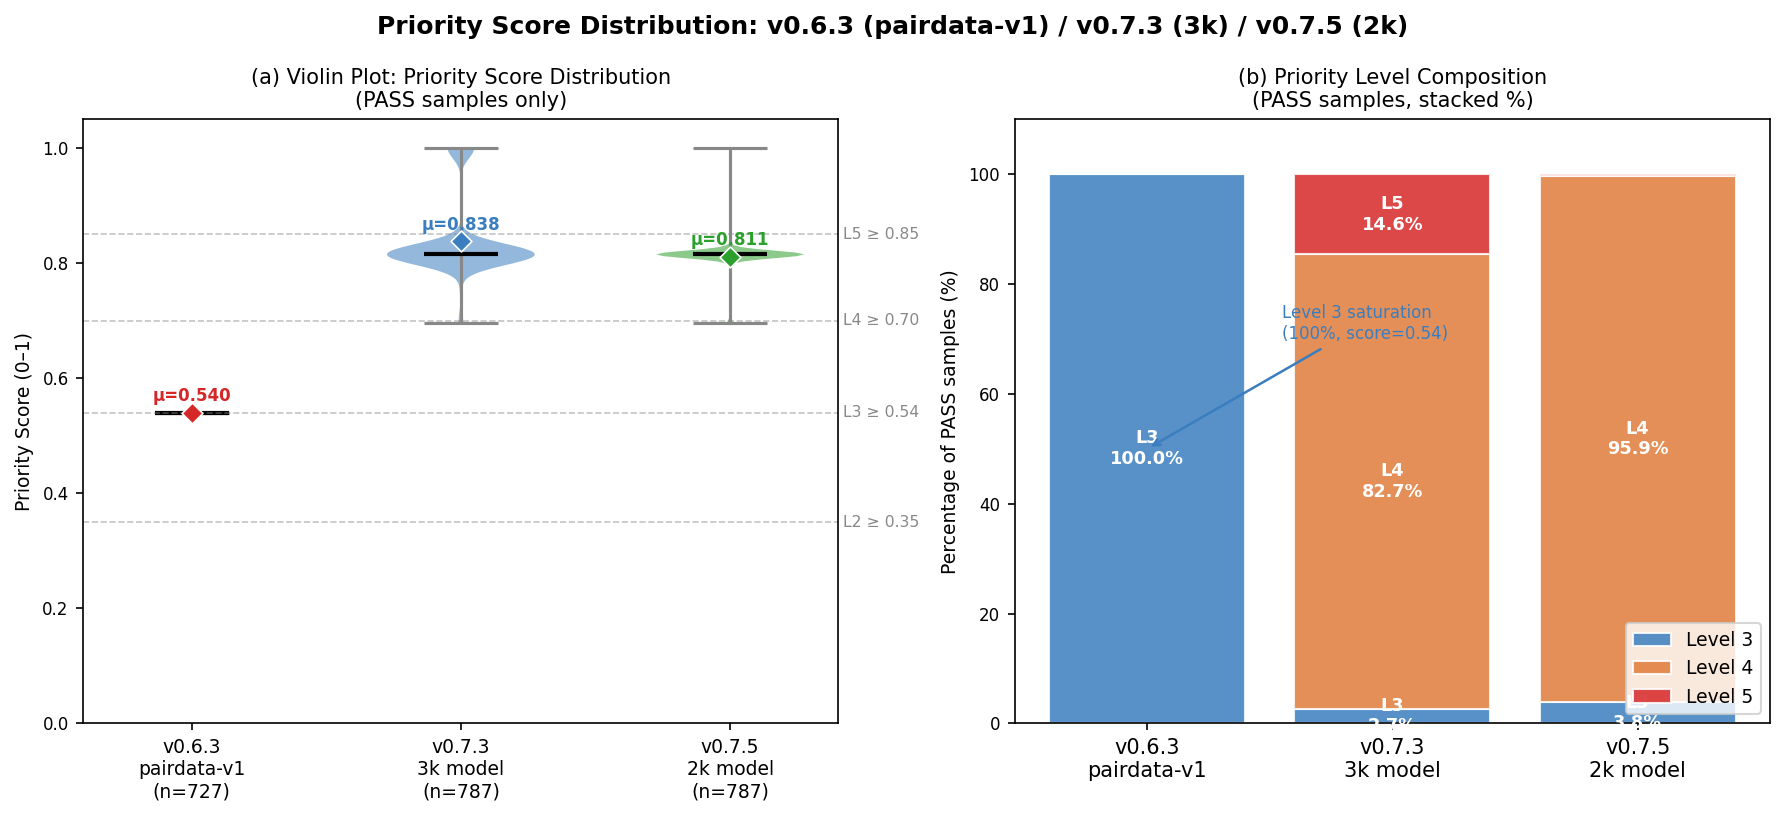
\includegraphics[width=0.9\textwidth]{figures_vlm/20_priority_score_violin.png}
\caption{Priority score distribution across three pipeline versions
         (PASS samples only).
         \textit{Left (a)}: violin plots with median (horizontal bar) and mean (diamond marker);
         dashed lines mark priority-level thresholds.
         \textit{Right (b)}: stacked percentage bars showing Level~3/4/5 composition.
         v0.6.3 collapses to a point mass at score~0.54 (Level~3, zero variance);
         both pairdata-v2 models restore score discriminability,
         concentrating mass in the Level~4 region
         ($\mu=0.838$ and $\mu=0.811$ for v0.7.3 and v0.7.5 respectively).}
\label{fig:s72_violin}
\end{figure}

The violin plot reveals a qualitative shift in the scoring distribution
across pipeline versions.
Under v0.6.3 (pairdata-v1), the priority score collapses to a point mass
at 0.54, producing a degenerate distribution with zero variance.
This confirms that the YAML rule engine, operating on mode-collapsed
model outputs, cannot distinguish severity levels within the PASS subset.

Both pairdata-v2 models exhibit broad, asymmetric distributions
spanning the Level~4 region (0.70--0.85).
The v0.7.3 3k model achieves mean score $\mu=0.838$ (std~0.070),
with a longer right tail extending into Level~5 ($\geq0.85$),
accounting for its 14.6\,\% Level~5 allocation.
The v0.7.5 2k model shows a narrower, more concentrated distribution
($\mu=0.811$, std~0.025), with scores tightly clustered around
the median (0.815), reflecting the 2k model's tendency to produce
medium-high severity vocabulary without the extreme-severity descriptors
that push scores above the Level~5 threshold.

This comparison demonstrates that both pairdata-v2 models successfully
restore score discriminability---from a point-mass degenerate distribution
to a Level~4-dominated spread---while exhibiting distinct variance
profiles driven by training duration.
The 2k model favors operational predictability (consistent Level~4
assignments, std~0.025), whereas the 3k model achieves higher severity
coverage at the cost of greater variability (std~0.070).
% ── S.8 Qualitative Analysis ─────────────────────────────────────────────
\clearpage
\section*{S.8\quad Qualitative Analysis: Representative PASS Predictions}
\label{sec:s8}

Figures~\ref{fig:s8_pass_1}--\ref{fig:s8_pass_3} present twelve representative PASS predictions for each of the two pipeline variants.
\textbf{Pred$_1$} is produced by the v0.7.5 pipeline (2k model); \textbf{Pred$_2$} is produced by the v0.7.3 pipeline (3k model), shown for comparison.
Both pipelines use Quality Guard $\theta_{\mathrm{low}}=30$, $\theta_{\mathrm{high}}=200$.
Images are selected to cover a range of structural members and damage types.
\textit{Sim(emb)} denotes the sentence-embedding cosine similarity for the 2k model output.
Shared damage/member terms between GT and Pred$_1$ (2k) are bold in Pred$_1$; terms shared between GT and Pred$_2$ (3k) are bold in Pred$_2$.

\begin{figure}[H]
  \centering
  \begin{minipage}[t]{0.46\textwidth}
    {\centering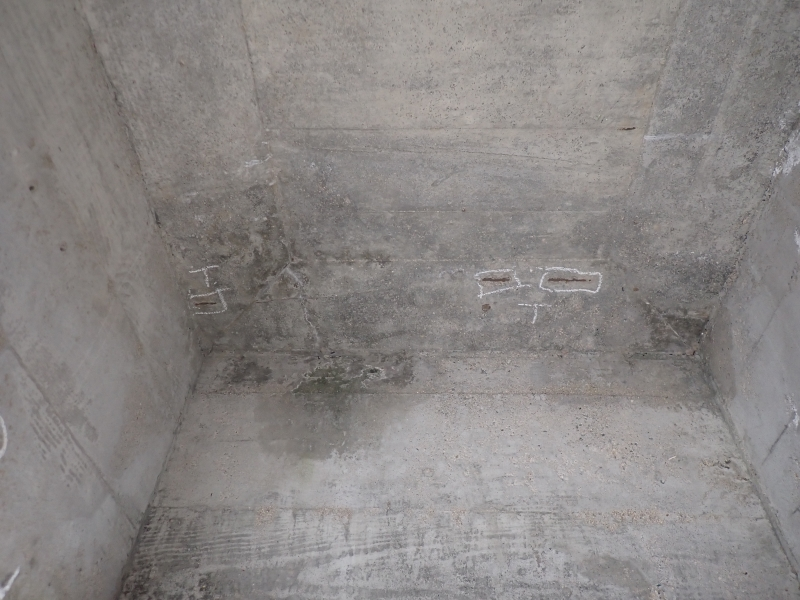
\includegraphics[width=0.675\linewidth]{figures_vlm/s8/s8_01_girder_cracking.jpg}\par}
    \vspace{2pt}
    {\scriptsize\raggedright
    \textbf{Quality Metrics (2k):}~\textit{Sim(emb):~0.552}\\[1pt]
    \textbf{GT:} \textbf{main girder} \textbf{cracking}(max W=0.6mm), \textbf{cross beam} \textbf{cracking}(max W=0.25mm), deck slab \textbf{cracking}(W=0.2mm); \textbf{lime \textbf{efflorescence}} observed. \textbf{cracking} , \textbf{drying shrinkage} ; ASR .\\[1pt]
    \textbf{Pred$_1$ (2k):} \textbf{main girder} \textbf{cracking}(max W=0.3mm); rebar exposure, \textbf{cross beam} delamination; rebar exposure observed. Also, filler zone \textbf{lime efflorescence} observed. parapet \textbf{drying shrinkage} water leakage, localized. periodic monitoring;, repair if necessary. rebar exposure, insufficient cover and carbonation.\\[1pt]
    \textbf{Pred$_2$ (3k):} \textbf{main girder} rebar exposure observed. Also, filler zone , \textbf{lime \textbf{efflorescence}} is present. localized , joint .
    \par}
  \end{minipage}
  \hfill
  \begin{minipage}[t]{0.46\textwidth}
    {\centering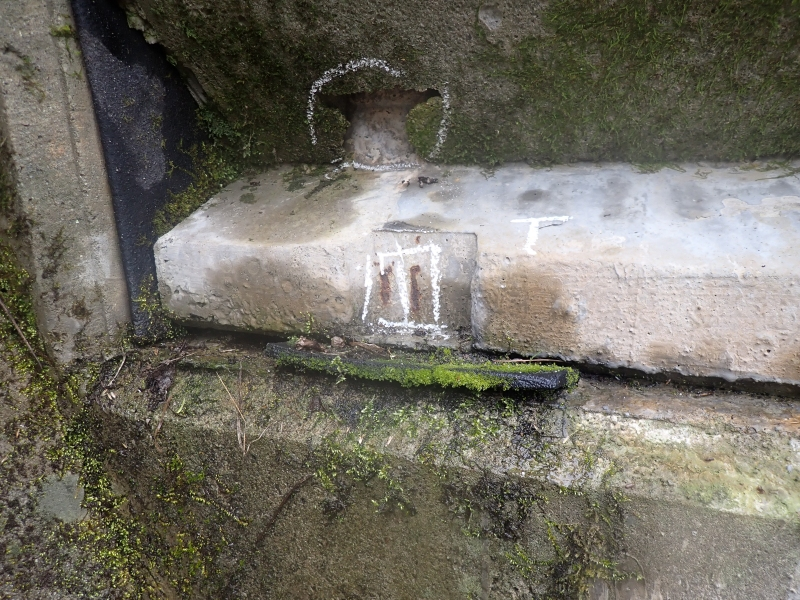
\includegraphics[width=0.675\linewidth]{figures_vlm/s8/s8_02_girder_rebar_exposure.jpg}\par}
    \vspace{2pt}
    {\scriptsize\raggedright
    \textbf{Quality Metrics (2k):}~\textit{Sim(emb):~0.418}\\[1pt]
    \textbf{GT:} RCT girder, \textbf{cross beam} and deck slab \textbf{delamination}, \textbf{rebar exposure} . \textbf{joint} \textbf{main girder} delamination . RCT girder and deck slab spalling corrosion .\\[1pt]
    \textbf{Pred$_1$ (2k):} \textbf{main girder} cracking(max W=0.3mm); \textbf{rebar exposure}, \textbf{cross beam} \textbf{delamination}; \textbf{rebar exposure} observed. localized. Also, parapet runoff water insufficient cover carbonation. \textbf{joint} and expansion joint.\\[1pt]
    \textbf{Pred$_2$ (3k):} \textbf{main girder} \textbf{rebar exposure} observed. Also, parapet/overhang \textbf{delamination} water leakage observed. parapet , drying shrinkage insufficient cover . localized .
    \par}
  \end{minipage}
  \\[4pt]
  \begin{minipage}[t]{0.46\textwidth}
    {\centering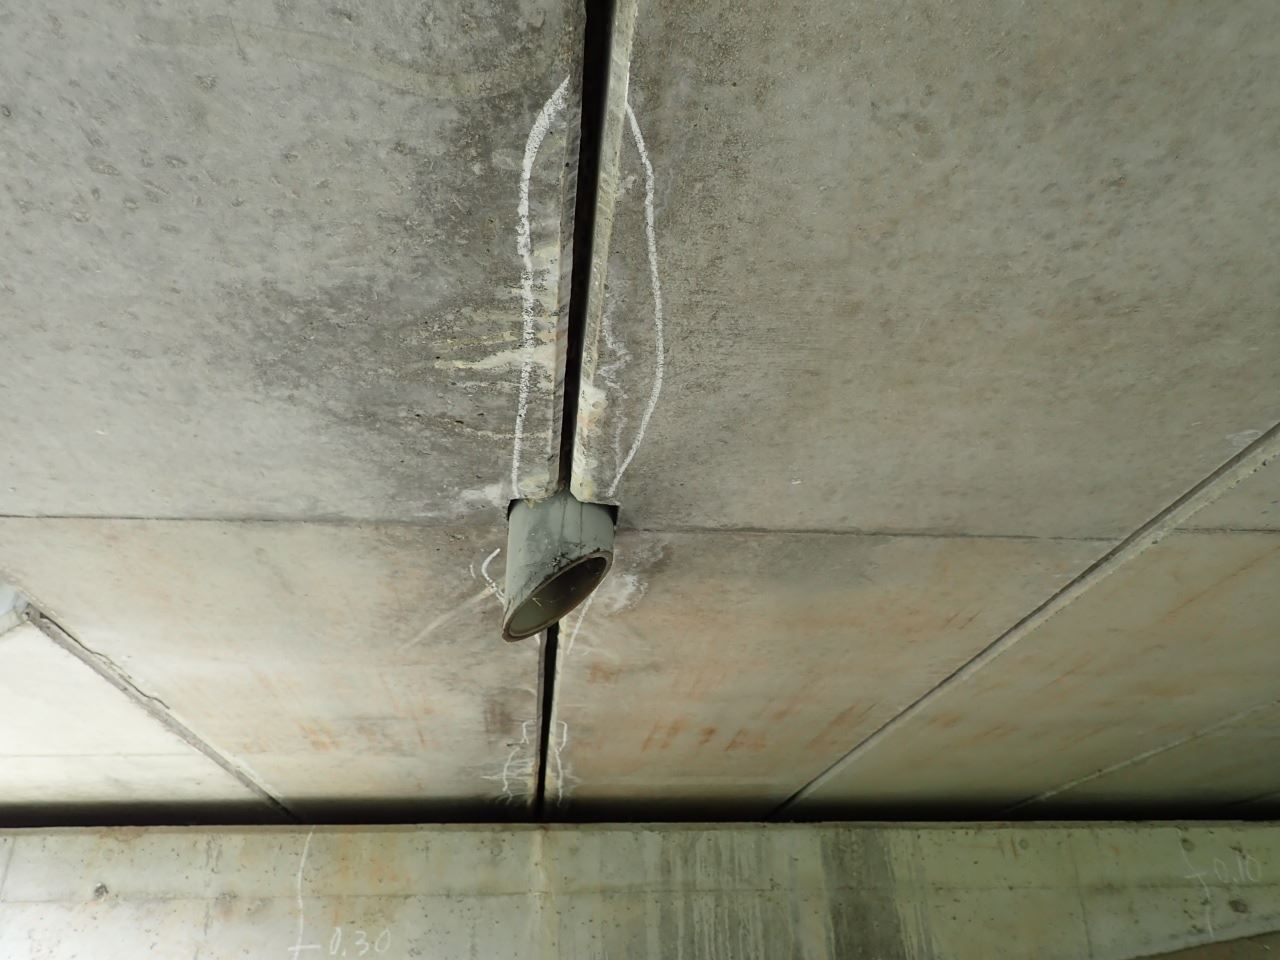
\includegraphics[width=0.675\linewidth]{figures_vlm/s8/s8_03_girder_spalling.jpg}\par}
    \vspace{2pt}
    {\scriptsize\raggedright
    \textbf{Quality Metrics (2k):}~\textit{Sim(emb):~0.658}\\[1pt]
    \textbf{GT:} \textbf{main girder} \textbf{delamination}, corrosion, water leakage trace observed. \textbf{repair} as needed.\\[1pt]
    \textbf{Pred$_1$ (2k):} \textbf{main girder} cracking(max W=0.3mm); rebar exposure, cross beam \textbf{delamination}; rebar exposure observed. localized. Also, parapet runoff water insufficient cover carbonation. periodic monitoring;, \textbf{repair} if necessary.\\[1pt]
    \textbf{Pred$_2$ (3k):} \textbf{main girder} rebar exposure observed. Also, parapet/overhang \textbf{delamination} rebar exposure observed. periodic monitoring;, repair if necessary .
    \par}
  \end{minipage}
  \hfill
  \begin{minipage}[t]{0.46\textwidth}
    {\centering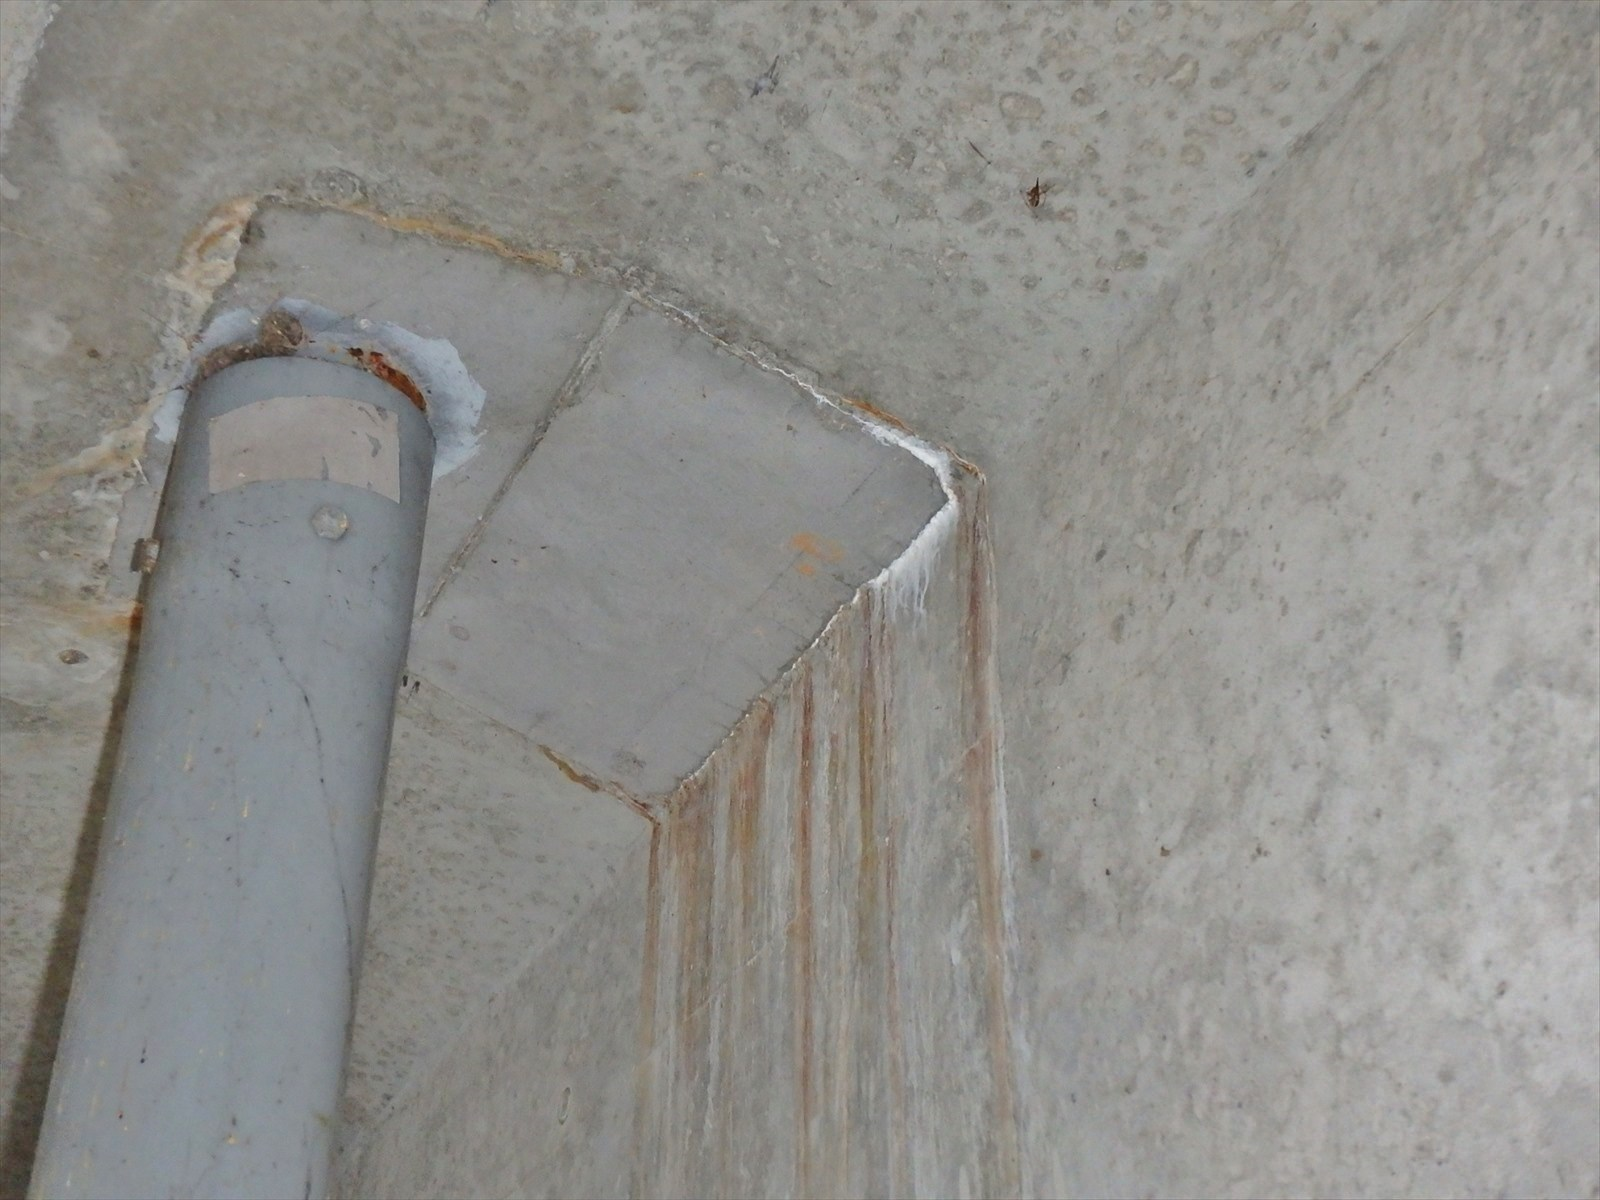
\includegraphics[width=0.675\linewidth]{figures_vlm/s8/s8_04_girder_corrosion.jpg}\par}
    \vspace{2pt}
    {\scriptsize\raggedright
    \textbf{Quality Metrics (2k):}~\textit{Sim(emb):~0.441}\\[1pt]
    \textbf{GT:} ; \textbf{main girder} expansion joint water leakage due tosection thinning \textbf{corrosion} observed. Also, splice bolt \textbf{corrosion} observed. ; \textbf{cross beam} age-related deterioration due to \textbf{corrosion} due to observed.\\[1pt]
    \textbf{Pred$_1$ (2k):} \textbf{main girder} cracking(max W=0.3mm); rebar exposure, \textbf{cross beam} delamination; rebar exposure observed. localized. Also, parapet runoff water \textbf{corrosion}.\\[1pt]
    \textbf{Pred$_2$ (3k):} \textbf{main girder} rebar exposure observed. Also, parapet/overhang delamination rebar exposure observed. periodic monitoring;, repair if necessary .
    \par}
  \end{minipage}
  \caption{Representative PASS predictions (1/3). Each panel: \textbf{GT} (original record), \textbf{Pred$_1$} (v0.7.5 2k model), \textbf{Pred$_2$} (v0.7.3 3k model, comparison). \textit{Sim(emb)} is for the 2k model. GT/Pred$_1$ shared terms bold in Pred$_1$; GT/Pred$_2$ shared terms bold in Pred$_2$.}
  \label{fig:s8_pass_1}
\end{figure}
\clearpage
\begin{figure}[H]
  \centering
  \begin{minipage}[t]{0.46\textwidth}
    {\centering\includegraphics[width=0.675\linewidth]{figures_vlm/s8/s8_05_girder_leakage.jpg}\par}
    \vspace{2pt}
    {\scriptsize\raggedright
    \textbf{Quality Metrics (2k):}~\textit{Sim(emb):~0.537}\\[1pt]
    \textbf{GT:} \textbf{main girder} \textbf{cracking} drying shrinkage due toage-related deterioration . \textbf{main girder} water leakage main girderjoint age-related deterioration .\\[1pt]
    \textbf{Pred$_1$ (2k):} \textbf{main girder} \textbf{cracking}(max W=0.25mm); rebar exposure, cross beam delamination; rebar exposure observed. localized. Also, parapet.\\[1pt]
    \textbf{Pred$_2$ (3k):} \textbf{main girder} rebar exposure observed. Also, parapet , (localized) .
    \par}
  \end{minipage}
  \hfill
  \begin{minipage}[t]{0.46\textwidth}
    {\centering\includegraphics[width=0.675\linewidth]{figures_vlm/s8/s8_06_girder_settlement.jpg}\par}
    \vspace{2pt}
    {\scriptsize\raggedright
    \textbf{Quality Metrics (2k):}~\textit{Sim(emb):~0.643}\\[1pt]
    \textbf{GT:} \textbf{expansion joint} deformation, P3 ; \textbf{main girder} , drainage basin sediment clogging observed. drainage basin , . , periodic monitoring;, \textbf{repair} if necessary .\\[1pt]
    \textbf{Pred$_1$ (2k):} \textbf{main girder} cracking(max W=0.3mm); rebar exposure, cross beam delamination; rebar exposure observed. localized. Also, parapet observed, \textbf{expansion joint}. \textbf{repair} as needed.\\[1pt]
    \textbf{Pred$_2$ (3k):} \textbf{main girder} cracking, delamination observed. Also, filler zone rust staining , progression monitoring required . parapet and guardrail rebar exposure , localized rebar exposure , periodic monitoring;, repair if necessary .
    \par}
  \end{minipage}
  \\[4pt]
  \begin{minipage}[t]{0.46\textwidth}
    {\centering\includegraphics[width=0.675\linewidth]{figures_vlm/s8/s8_07_girder_other.jpg}\par}
    \vspace{2pt}
    {\scriptsize\raggedright
    \textbf{Quality Metrics (2k):}~\textit{Sim(emb):~0.593}\\[1pt]
    \textbf{GT:} \textbf{main girder} \textbf{cracking}, \textbf{delamination} observed. \textbf{repair} is recommended.\\[1pt]
    \textbf{Pred$_1$ (2k):} \textbf{main girder} \textbf{cracking}(max W=0.3mm); rebar exposure, cross beam \textbf{delamination}; rebar exposure observed. localized, periodic monitoring;, \textbf{repair} if necessary. Also, expansion joint water leakage.\\[1pt]
    \textbf{Pred$_2$ (3k):} \textbf{main girder} rebar exposure, \textbf{delamination} observed. Also, parapet/overhang observed. periodic monitoring;, repair if necessary . , expansion joint water leakage .
    \par}
  \end{minipage}
  \hfill
  \begin{minipage}[t]{0.46\textwidth}
    {\centering\includegraphics[width=0.675\linewidth]{figures_vlm/s8/s8_08_slab_cracking.jpg}\par}
    \vspace{2pt}
    {\scriptsize\raggedright
    \textbf{Quality Metrics (2k):}~\textit{Sim(emb):~0.700}\\[1pt]
    \textbf{GT:} PC slab bridge rubber bearing \textbf{cracking}, deformation was observed.\\[1pt]
    \textbf{Pred$_1$ (2k):} main girder \textbf{cracking}(max W=0.3mm); rebar exposure, cross beam delamination; rebar exposure observed. localized. Also, parapet runoff water insufficient cover carbonation. periodic monitoring;, repair if necessary.\\[1pt]
    \textbf{Pred$_2$ (3k):} main girder rebar exposure observed. Also, generallywater leakage; lime efflorescence , parapet runoff water drying shrinkage due to \textbf{cracking} . rebar exposure insufficient cover carbonation .
    \par}
  \end{minipage}
  \caption{Representative PASS predictions (2/3). Each panel: \textbf{GT} (original record), \textbf{Pred$_1$} (v0.7.5 2k model), \textbf{Pred$_2$} (v0.7.3 3k model, comparison). \textit{Sim(emb)} is for the 2k model. GT/Pred$_1$ shared terms bold in Pred$_1$; GT/Pred$_2$ shared terms bold in Pred$_2$.}
  \label{fig:s8_pass_2}
\end{figure}
\clearpage
\begin{figure}[H]
  \centering
  \begin{minipage}[t]{0.46\textwidth}
    {\centering\includegraphics[width=0.675\linewidth]{figures_vlm/s8/s8_09_slab_rebar_exposure.jpg}\par}
    \vspace{2pt}
    {\scriptsize\raggedright
    \textbf{Quality Metrics (2k):}~\textit{Sim(emb):~0.555}\\[1pt]
    \textbf{GT:} \textbf{deck slab} \textbf{cracking} was observed. Also, due to\textbf{rebar exposure} was observed , monitoring is required.\\[1pt]
    \textbf{Pred$_1$ (2k):} main girder \textbf{cracking}(max W=0.3mm); \textbf{rebar exposure}, cross beam delamination; \textbf{rebar exposure} observed. localized. Also, parapet runoff water insufficient cover carbonation. periodic monitoring;, repair if necessary.\\[1pt]
    \textbf{Pred$_2$ (3k):} main girder \textbf{cracking}, delamination, \textbf{rebar exposure} observed. \textbf{deck slab} localized rebar exposure , . expansion joint parapet runoff water .
    \par}
  \end{minipage}
  \hfill
  \begin{minipage}[t]{0.46\textwidth}
    {\centering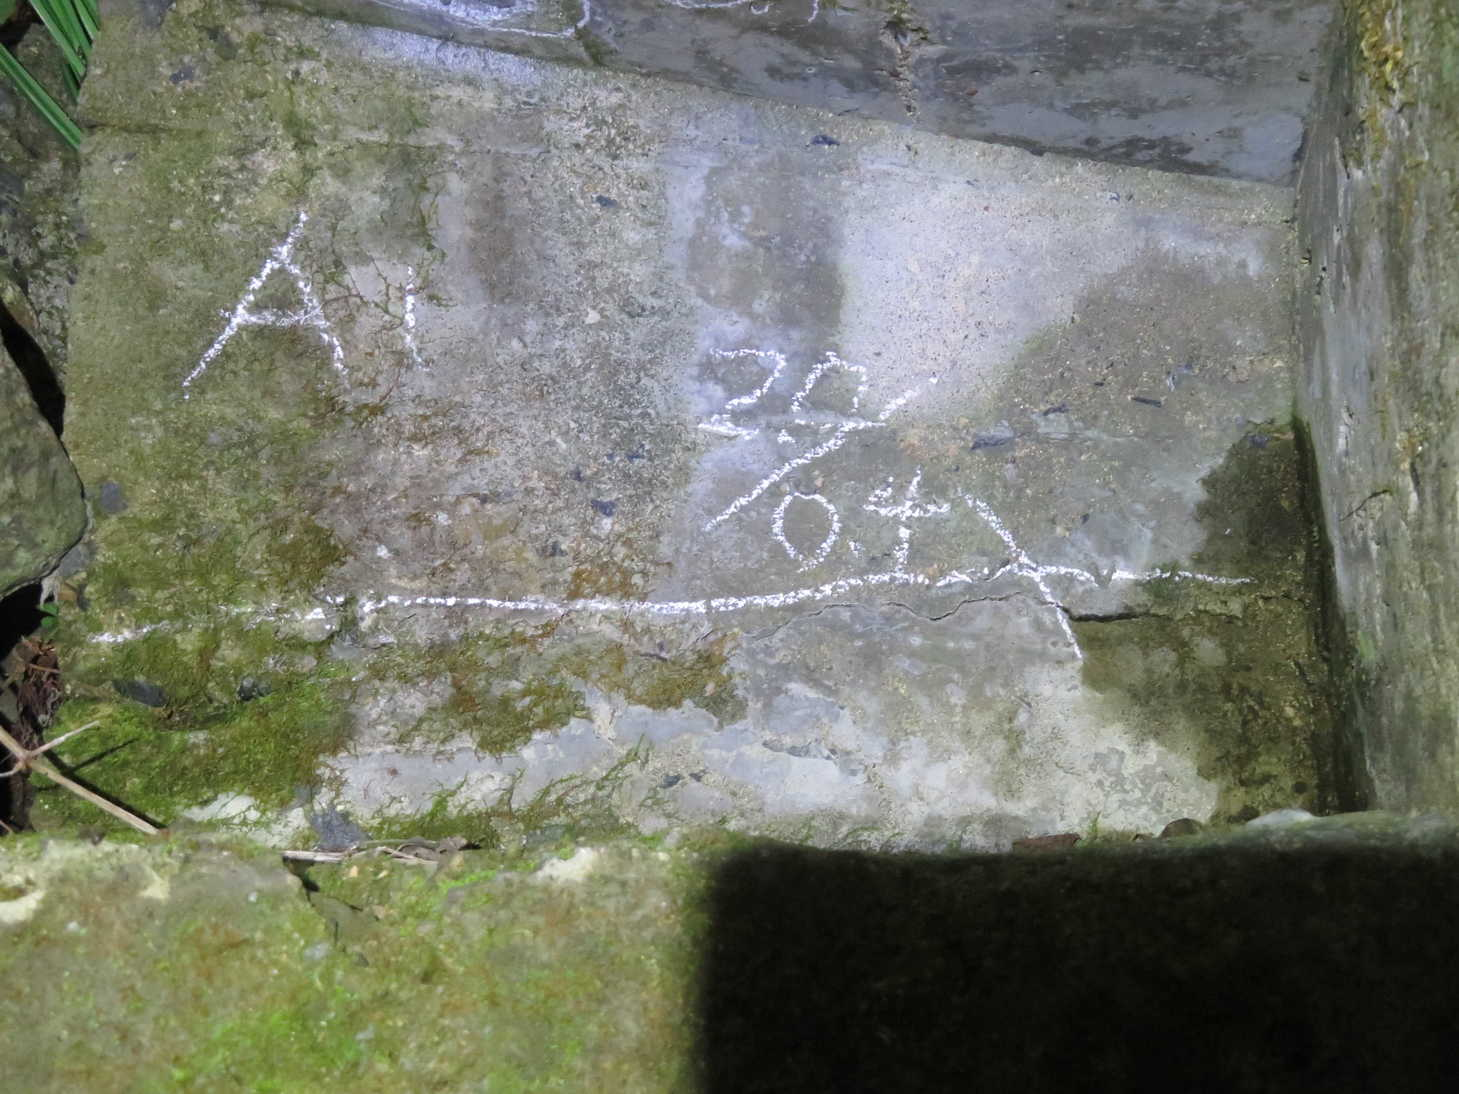
\includegraphics[width=0.675\linewidth]{figures_vlm/s8/s8_10_abutment_cracking.jpg}\par}
    \vspace{2pt}
    {\scriptsize\raggedright
    \textbf{Quality Metrics (2k):}~\textit{Sim(emb):~0.770}\\[1pt]
    \textbf{GT:} A1abutment \textbf{cracking}(max W=1.2mm); lime efflorescence, P1pier \textbf{cracking}(max W=0.3mm); rust staining lime efflorescence; , A1abutment; P1pier \textbf{expansion joint} \textbf{water leakage} trace observed. \textbf{cracking} rust staining and localized , \textbf{periodic monitoring};, \textbf{repair} if necessary .\\[1pt]
    \textbf{Pred$_1$ (2k):} main girder \textbf{cracking}(max W=0.3mm); rebar exposure, cross beam delamination; rebar exposure observed. Also, parapet \textbf{expansion joint} \textbf{water leakage} due to insufficient cover observed. age-related deterioration drying shrinkage. \textbf{periodic monitoring};, \textbf{repair} if necessary.\\[1pt]
    \textbf{Pred$_2$ (3k):} main girder rebar exposure observed. Also, parapet/overhang delamination \textbf{water leakage} is present. parapet delamination , insufficient cover carbonation . localized .
    \par}
  \end{minipage}
  \\[4pt]
  \begin{minipage}[t]{0.46\textwidth}
    {\centering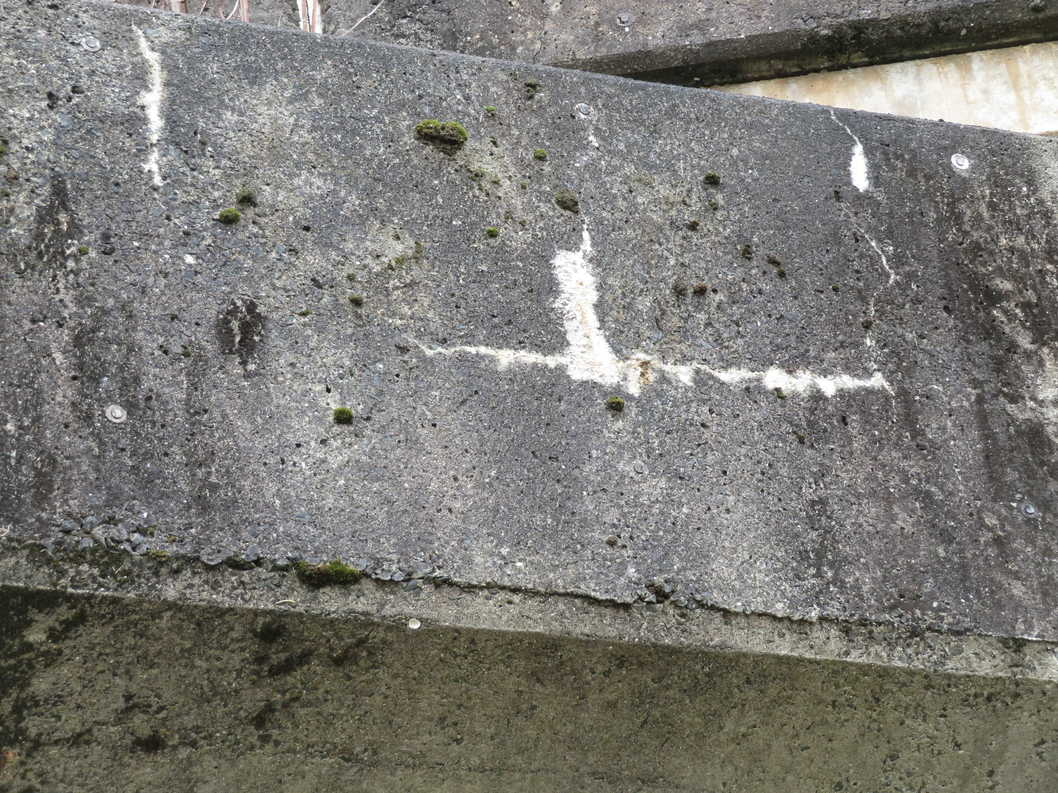
\includegraphics[width=0.675\linewidth]{figures_vlm/s8/s8_11_abutment_rebar_exposure.jpg}\par}
    \vspace{2pt}
    {\scriptsize\raggedright
    \textbf{Quality Metrics (2k):}~\textit{Sim(emb):~0.798}\\[1pt]
    \textbf{GT:} abutment, pier \textbf{cracking}, \textbf{rebar exposure}, water leakage trace observed. from a durability standpoint,\textbf{repair} is recommended.\\[1pt]
    \textbf{Pred$_1$ (2k):} main girder \textbf{cracking}(max W=0.3mm); \textbf{rebar exposure}, cross beam delamination; \textbf{rebar exposure} observed. Also, parapet expansion joint infiltration water due to rust staining. localized, periodic monitoring;, \textbf{repair} if necessary.\\[1pt]
    \textbf{Pred$_2$ (3k):} main girder \textbf{rebar exposure} observed. Also, generally\textbf{cracking} delamination , expansion joint infiltration water internal rebar expansion .
    \par}
  \end{minipage}
  \hfill
  \begin{minipage}[t]{0.46\textwidth}
    {\centering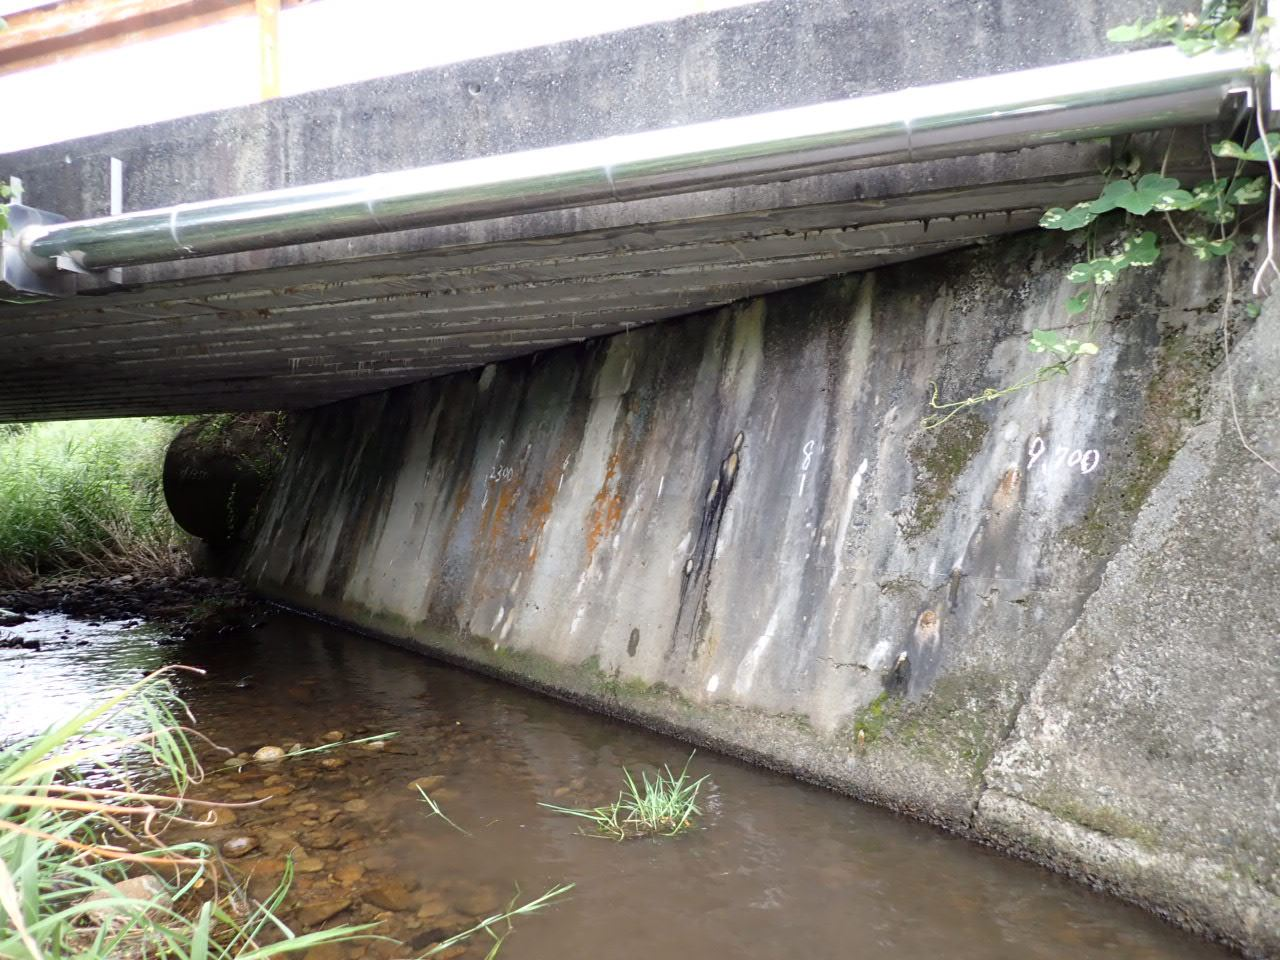
\includegraphics[width=0.675\linewidth]{figures_vlm/s8/s8_12_abutment_spalling.jpg}\par}
    \vspace{2pt}
    {\scriptsize\raggedright
    \textbf{Quality Metrics (2k):}~\textit{Sim(emb):~0.656}\\[1pt]
    \textbf{GT:} abutment honeycombing spalling is present. \textbf{bearing} soil ejection, lime efflorescence water leakage trace observed. abutment honeycombing , rust staining water leakage trace observed. observed.\\[1pt]
    \textbf{Pred$_1$ (2k):} main girder cracking(max W=0.3mm); rebar exposure, cross beam delamination; rebar exposure observed. localized, periodic monitoring;, repair if necessary. Also, parapet runoff water corrosion.\\[1pt]
    \textbf{Pred$_2$ (3k):} main girder rebar exposure, delamination observed. Also, parapet/overhang , expansion joint infiltration water \textbf{bearing} . periodic monitoring;, repair if necessary . , expansion joint infiltration water due to .
    \par}
  \end{minipage}
  \caption{Representative PASS predictions (3/3). Each panel: \textbf{GT} (original record), \textbf{Pred$_1$} (v0.7.5 2k model), \textbf{Pred$_2$} (v0.7.3 3k model, comparison). \textit{Sim(emb)} is for the 2k model. GT/Pred$_1$ shared terms bold in Pred$_1$; GT/Pred$_2$ shared terms bold in Pred$_2$.}
  \label{fig:s8_pass_3}
\end{figure}

\noindent When damage/member keywords appear in \emph{both} GT and Pred$_2$ (3k), \textit{Sim(emb)} is correspondingly high, indicating successful damage recognition. Pred$_1$ (2k) consistently includes cross beam (98.3\,\% rate) and the cracking--rebar-exposure compound descriptor, reflecting the 2k model's template-driven vocabulary. Conversely, terms present only in GT are absent from both predictions---representing the remaining recognition gap and a direction for future improvement.

\end{document}
